\documentclass[twoside,10pt]{book}
\usepackage[amsbb,mtpfrak,zswash,mtpcal]{mtpro2}
\usepackage[no-math,cm-default]{fontspec}
\usepackage{xunicode}
\usepackage{xltxtra}
\usepackage{xgreek}
\defaultfontfeatures{Mapping=tex-text,Scale=MatchLowercase}
\setmainfont[Mapping=tex-text,Numbers=Lining,Scale=1.0,BoldFont={Minion Pro Bold}]{Minion Pro}
\defaultfontfeatures{Ligatures=TeX}
\font\kefalaio="Minion Pro Bold" at 36pt
\font\ArKef="Minion Pro Bold Italic" at 72pt
\font\OnKef="Times New Roman" at 20pt
\font\OnPar="Minion Pro Bold" at 18pt
\newfontfamily\scfont{GFS Artemisia}
\usepackage[inner=2.00cm, outer=1.50cm, top=3.00cm, bottom=2.00cm,paperwidth=17cm,paperheight=24cm]{geometry}
\usepackage{amsmath}
\usepackage[amsbb,mtpfrak,zswash,mtpcal]{mtpro2}
\usepackage{makeidx}
\usepackage{longtable,xcolor}
\def\xrwma{red!80!black}
\def\xrwmath{red}
\usepackage{etoolbox}
\makeatletter
\newif\ifLT@nocaption
\preto\longtable{\LT@nocaptiontrue}
\appto\endlongtable{%
\ifLT@nocaption
\addtocounter{table}{\m@ne}%
\fi}
\preto\LT@caption{%
\noalign{\global\LT@nocaptionfalse}}
\makeatother
\makeindex
\usepackage{tikz,pgfplots}
\usepackage{tkz-euclide,tkz-fct}
\usetikzlibrary{fadings}
\usepackage{wrap-rl}
\usetkzobj{all}
\usepackage{calc}
\usepackage{cleveref}
\usepackage[colorlinks=false, pdfborder={0 0 0}]{hyperref}
\usepackage[framemethod=TikZ]{mdframed}
\definecolor{steelblue}{cmyk}{.7,.278,0,.294}
\definecolor{doc}{cmyk}{1,0.455,0,0.569}
\definecolor{olivedrab}{cmyk}{0.25,0,0.75,0.44}
\usepackage{capt-of}
\usepackage{titletoc}
\usepackage[explicit]{titlesec}
\usepackage{graphicx}
\usepackage{multicol}
\usepackage{multirow}
\usepackage{enumitem}
\usepackage{tabularx}
\usepackage[decimalsymbol=comma]{siunitx}
\tikzset{>=latex}
\makeatletter
\pretocmd{\@part}{\gdef\parttitle{#1}}{}{}
\pretocmd{\@spart}{\gdef\parttitle{#1}}{}{}
\makeatother
\usepackage[titletoc]{appendix}
\usepackage{fancyhdr}
\pagestyle{fancy}
\fancyheadoffset{0cm}
\renewcommand{\headrulewidth}{\iftopfloat{0pt}{.5pt}}
\renewcommand{\chaptermark}[1]{\markboth{#1}{}}
\renewcommand{\sectionmark}[1]{\markright{\it\thesection\ #1}}
\fancyhf{}
\fancyhead[LE]{\thepage\ $\cdot$\ \scfont\scshape\nouppercase{\leftmark}}
\fancyhead[RO]{\nouppercase{\rightmark} $\cdot$\ \thepage}
\fancypagestyle{plain}{%
\fancyhead{} %
\renewcommand{\headrulewidth}{0pt}}

\newcounter{thewrhma}[chapter]
\renewcommand{\thethewrhma}{\thechapter.\arabic{thewrhma}} 
\newcommand{\Thewrhma}[1]{\refstepcounter{thewrhma}{\textbf{\textcolor{\xrwmath}{{\large Θεώρημα\hspace{2mm}\thethewrhma\;}:\;}\hspace{1mm}}} \MakeUppercase{\textbf{#1}}\\}{}

\newcounter{porisma}[chapter]
\renewcommand{\theporisma}{\thechapter.\arabic{porisma}}\newcommand{\Porisma}[1]{\refstepcounter{porisma}\textcolor{black}{\textbf{ΠΟΡΙΣΜΑ\hspace{2mm}\theporisma\hspace{1mm} \MakeUppercase{#1}}}\\}{}

\newcounter{protasi}[chapter]
\renewcommand{\theprotasi}{\thechapter.\arabic{protasi}}\newcommand{\Protasi}[1]{\refstepcounter{protasi}\textcolor{black}{\textbf{ΠΡΟΤΑΣΗ\hspace{2mm}\theprotasi\hspace{1mm} \MakeUppercase{#1}}}\\}{}


\newcounter{orismos}[section]
\renewcommand{\theorismos}{\arabic{orismos}}   
\newcommand{\Orismos}[1]{\refstepcounter{orismos}{\textbf{\textbf{\textcolor{\xrwma}{{\large Ορισμός\hspace{2mm}\theorismos\;}:\;}}}}\hspace{1mm} \MakeUppercase{\textbf{#1}\\}}{}
\usepackage{venndiagram,mathimatika}
%-------- ΣΤΥΛ ΚΕΦΑΛΑΙΟΥ ---------
\newcommand*\chapterlabel{}
\newcommand{\fancychapter}{%
\titleformat{\chapter}
{
\normalfont\Huge}
{\gdef\chapterlabel{\thechapter\ }}{0pt}
{\begin{tikzpicture}[remember picture,overlay]
\node[yshift=-7cm] at (current page.north west)
{\begin{tikzpicture}[remember picture, overlay]
%\node[inner sep=0pt] at ($(current page.north) +			(0cm,-1.38in)$) {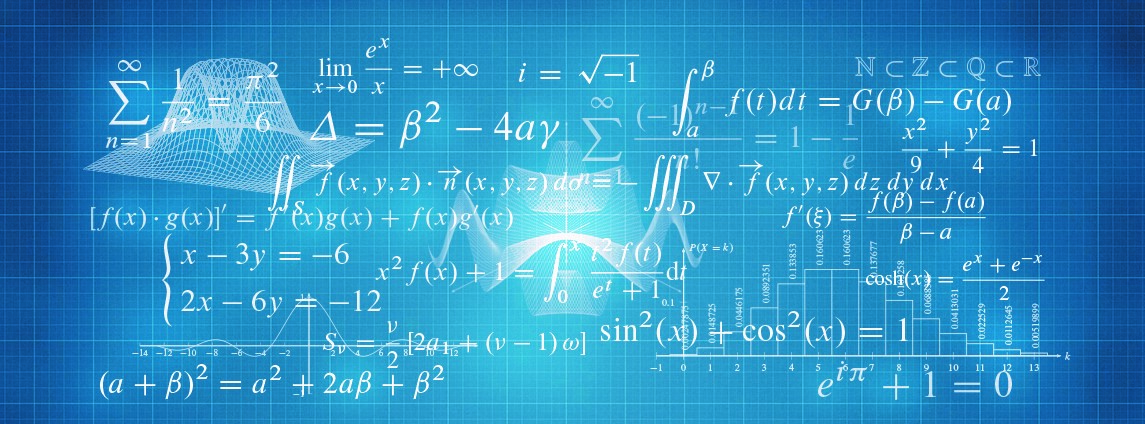
\includegraphics[width=17cm]{Kefalaio}};
\node[anchor=west,xshift=.1\paperwidth,yshift=.14\paperheight,rectangle]
{{\color{white}\fontsize{30}{20}\textbf{\textcolor{black}{\contour{white}{ΚΕΦΑΛΑΙΟ}}}}};
\node[anchor=west,xshift=.09\paperwidth,yshift=.08\paperheight,rectangle] {\fontsize{24}{20} {\color{black}{{\textcolor{black}{\contour{white}{\sc##1}}}}}};
%\fill[fill=black] (12.2,2) rectangle (14.8,4.7);
\node[anchor=west,xshift=.74\paperwidth,yshift=.11\paperheight,rectangle]
{{\color{white}\fontsize{80}{20}\textbf{\textit{\textcolor{white}{\contour{black}{\thechapter}}}}}};
\end{tikzpicture}
};
\end{tikzpicture}
}
\titlespacing*{\chapter}{0pt}{20pt}{30pt}
}
%------------------------------------------------


\usepackage[outline]{contour}
\newcommand{\regularchapter}{%
\titleformat{\chapter}[display]
{\normalfont\huge\bfseries}{\chaptertitlename\ \thechapter}{20pt}{\Huge##1}
\titlespacing*{\chapter}
{0pt}{-20pt}{40pt}
}

\apptocmd{\mainmatter}{\fancychapter}{}{}
\apptocmd{\backmatter}{\regularchapter}{}{}
\apptocmd{\frontmatter}{\regularchapter}{}{}

\titlespacing*{\section}
{0pt}{30pt}{0pt}
\usepackage{booktabs}
\usepackage{hhline}
\DeclareRobustCommand{\perthousand}{%
\ifmmode
\text{\textperthousand}%
\else
\textperthousand
\fi}


\contentsmargin{0cm}
\titlecontents{part}[-1pc]
{\addvspace{10pt}%
\bf\Large ΜΕΡΟΣ\quad }%
{}
{}
{\;\dotfill}%
%------------------------------------------
\titlecontents{chapter}[0pc]
{\addvspace{30pt}%
\begin{tikzpicture}[remember picture, overlay]%
\draw[fill=black,draw=black] (-.3,.5) rectangle (3.7,1.1); %
\pgftext[left,x=0cm,y=0.75cm]{\color{white}\sc\Large\bfseries Κεφάλαιο\ \thecontentslabel};%
\end{tikzpicture}\large\sc}%
{}
{}
{\hspace*{-2.3em}\hfill\normalsize Σελίδα \thecontentspage}%
\titlecontents{section}[2.4pc]
{\addvspace{1pt}}
{\contentslabel[\thecontentslabel]{2pc}}
{}
{\;\dotfill\;\small \thecontentspage}
[]
\titlecontents*{subsection}[4pc]
{\addvspace{-1pt}\small}
{}
{}
{\ --- \small\thecontentspage}
[ \textbullet\ ][]

\makeatletter
\renewcommand{\tableofcontents}{%
\chapter*{%
\vspace*{-20\p@}%
\begin{tikzpicture}[remember picture, overlay]%
\pgftext[right,x=12cm,y=0.2cm]{\Huge\sc\bfseries \contentsname};%
\draw[fill=black,draw=black] (9.5,-.75) rectangle (12.5,1);%
\clip (9.5,-.75) rectangle (15,1);
\pgftext[right,x=12cm,y=0.2cm]{\color{white}\Huge\bfseries \contentsname};%
\end{tikzpicture}}%
\@starttoc{toc}}
\makeatother

\usepackage[contents={},scale=1,opacity=1,color=black,angle=0]{background}

\newcommand\blfootnote[1]{%
\begingroup
\renewcommand\thefootnote{}\footnote{#1}%
\addtocounter{footnote}{-1}%
\endgroup
}
\usepackage{epstopdf}
\epstopdfsetup{update}
\usepackage{textcomp}

\titleformat{\section}
{\normalfont\Large\bf}%
{}{0em}%
{{\color{black}\titlerule[0pt]}\vskip-.2\baselineskip{\parbox[t]{\dimexpr\textwidth-2\fboxsep\relax}{\raggedright\strut\itshape{\LARGE{\thesection~#1}}\strut}}}[\vskip 0\baselineskip{\color{black}\titlerule[1pt]}]
\titlespacing*{\section}{0pt}{0pt}{30pt}

\newcommand{\methodologia}{\begin{center}
{\large \textbf{ΜΕΘΟΔΟΛΟΓΙΑ}}\\\vspace{-2mm}
\begin{tikzpicture}
\shade[left color=white, right color=black,] (-3cm,0) rectangle (0,.2mm);
\shade[left color=black, right color=white,] (0,0) rectangle (3cm,.2mm);   
\end{tikzpicture}
\end{center}}

\newcommand{\orismoi}{\begin{center}
\vspace{-3mm}{\large \textbf{\textcolor{\xrwma}{ΟΡΙΣΜΟΙ}}}\\\vspace{-2mm}
\begin{tikzpicture}
\shade[left color=white, right color=cyan!80!black,] (-3cm,0) rectangle (0,.2mm);
\shade[left color=cyan!80!black, right color=white,] (0,0) rectangle (3cm,.2mm);   
\end{tikzpicture}
\end{center}}
\newcommand{\thewrhmata}{\begin{center}
{\large \textbf{\textcolor{\xrwmath}{ΘΕΩΡΗΜΑΤΑ - ΠΟΡΙΣΜΑΤΑ - ΠΡΟΤΑΣΕΙΣ\\ΚΡΙΤΗΡΙΑ - ΙΔΙΟΤΗΤΕΣ}}}\\\vspace{-2mm}
\begin{tikzpicture}
\shade[left color=white, right color=\xrwmath,] (-5cm,0) rectangle (0,.2mm);
\shade[left color=\xrwmath, right color=white,] (0,0) rectangle (5cm,.2mm);   
\end{tikzpicture}
\end{center}}
\usepackage[labelfont={footnotesize,it,bf},font={footnotesize}]{caption}

%-------- ΠΙΝΑΚΕΣ ---------
\usepackage{booktabs}
%----------------------
%----- ΥΠΟΛΟΓΙΣΤΗΣ ----------
%\usepackage{calculator}
%----------------------------

%----- ΟΡΙΖΟΝΤΙΑ ΛΙΣΤΑ ------
\usepackage{xparse}
\newcounter{answers}
\renewcommand\theanswers{\arabic{answers}}
\ExplSyntaxOn
\NewDocumentCommand{\results}{m}
{
\seq_set_split:Nnn \l_results_a_seq {,}{#1}
\par\nobreak\noindent\setcounter{answers}{0}
\seq_map_inline:Nn \l_results_a_seq
{
\makebox[.18\linewidth][l]{\stepcounter{answers}\theanswers.~##1}\hfill
}
\par
}
\seq_new:N \l_results_a_seq
\ExplSyntaxOff
%----------------------------
%------ ΜΗΚΟΣ ΓΡΑΜΜΗΣ ΚΛΑΣΜΑΤΟΣ ---------
\DeclareRobustCommand{\frac}[3][0pt]{%
{\begingroup\hspace{#1}#2\hspace{#1}\endgroup\over\hspace{#1}#3\hspace{#1}}}
%----------------------------------------
\usepackage{microtype}
\usepackage{float}

\usepackage{caption}

%---- ΟΡΙΖΟΝΤΙΟ - ΚΑΤΑΚΟΡΥΦΟ - ΠΛΑΓΙΟ ΑΓΚΙΣΤΡΟ ------
\newcommand{\orag}[3]{\node at (#1)
{$ \overcbrace{\rule{#2mm}{0mm}}^{{\scriptsize #3}} $};}

\newcommand{\kag}[3]{\node at (#1)
{$ \undercbrace{\rule{#2mm}{0mm}}_{{\scriptsize #3}} $};}

\newcommand{\Pag}[4]{\node[rotate=#1] at (#2)
{$ \overcbrace{\rule{#3mm}{0mm}}^{{\rotatebox{-#1}{\scriptsize$#4$}}}$};}
%-----------------------------------------
\tikzstyle{pl}=[line width=0.3mm]
\tikzstyle{plm}=[line width=0.4mm]
%------- ΣΤΥΛ ΠΑΡΑΔΕΙΓΜΑΤΟΣ -------
\newcounter{paradeigma}[section]
\renewcommand{\theparadeigma}{\bf\arabic{paradeigma}\;:\;}   
\newcommand{\Paradeigma}[1]{\refstepcounter{paradeigma}\textcolor{black}{\textbf{ΠΑΡΑΔΕΙΓΜΑ\hspace{2mm}\theparadeigma\hspace{1mm}}} \MakeUppercase{\textbf{#1}}\\}{}
%-----------------------------------

%------- ΣΤΥΛ ΛΥΣΗΣ ------------------
\newcommand{\lysh}{{\textbf{ΛΥΣΗ}}}
%------------------------------------

%------ ΛΥΜΕΝΑ ΠΑΡΑΔΕΙΓΜΑΤΑ ΤΙΤΛΟΣ ---------
\newcommand{\Lymena}{\begin{center}
\begin{tikzpicture}
\fill[black] (-7cm,-.6cm) rectangle (6.5cm,.6cm);
\node at (-.25cm,0) {\Large \textcolor{white}{\textbf{ΛΥΜΕΝΑ ΠΑΡΑΔΕΙΓΜΑΤΑ}}};  
\end{tikzpicture}
\end{center}}
%--------------------------------------

%--------- ΑΛΥΤΕΣ ΑΣΚΗΣΕΙΣ ΤΙΤΛΟΣ ----------
\newcommand{\Alyta}{\begin{center}
\begin{tikzpicture}
\fill[black] (-7cm,-.6cm) rectangle (6.5cm,.6cm);
\node at (-.25cm,0) {\Large \textcolor{white}{\textbf{ΑΣΚΗΣΕΙΣ - ΠΡΟΒΛΗΜΑΤΑ}}};  
\end{tikzpicture}
\end{center}}
%--------------------------------------------
%---------- ΜΕΘΟΔΟΣ --------------
\newcounter{Methodos}[section]
\renewcommand{\theMethodos}{\thechapter.\arabic{Methodos}} 
\usepackage{varwidth}
\usetikzlibrary{calc}
\makeatletter
\newenvironment{Methodos}[2][\linewidth]
{\refstepcounter{Methodos}
\begin{mdframed}[
skipabove=\topsep,
skipbelow=\topsep,
roundcorner=2pt,
shadowsize=5pt,
linewidth=.8pt,
linecolor=black,
frametitle=\phantom{#1},
frametitlebelowskip=10pt,
innerleftmargin=12pt,
innerrightmargin=12pt,
frametitlefont=\large\bfseries\color{black},
singleextra={
\path[draw=black,left color=red!80!black,
right color=red] [rounded corners=2pt]
([xshift=.4pt,yshift=-\pgflinewidth+.1mm]O|-P.north west) to
([xshift=.4pt,yshift=-21pt]O|-P.north west) --
([xshift=-#2 -.7cm,yshift=-21pt]P.south east) --
([xshift=-#2,yshift=-\pgflinewidth+.1mm]P.north east) -- cycle;
\path let \p1=(P), \p2= (O) in 
node at ([xshift=-3mm,yshift=-11pt]0.5*\x1+0.5*\x2,\y1) {\parbox{\dimexpr\mdf@userdefinedwidth@length-40pt\relax
}{\bf\textcolor{white}{{\large Μέθοδος\hspace{2mm}\theMethodos\;:\;}} #1}};
}]}
{\end{mdframed}}
\makeatother
%------------------------------------------
%---------- ΛΙΣΤΕΣ ----------------------
\newlist{bhma}{enumerate}{3}
\setlist[bhma]{label=\bf\textit{\arabic*\textsuperscript{o}\;Βήμα :},leftmargin=0cm,itemindent=1.5cm,ref=\bf{\arabic*\textsuperscript{o}\;Βήμα}}
\newlist{rlist}{enumerate}{3}
\setlist[rlist]{itemsep=0mm,label=\roman*.}
\newlist{brlist}{enumerate}{3}
\setlist[brlist]{itemsep=0mm,label=\bf\roman*.}
\newlist{tropos}{enumerate}{3}
\setlist[tropos]{label=\bf\textit{\arabic*\textsuperscript{oς}\;Τρόπος :},leftmargin=0cm,itemindent=2.3cm,ref=\bf{\arabic*\textsuperscript{oς}\;Τρόπος}}
% Αν μπει το bhma μεσα σε tropo τότε
%\begin{bhma}[leftmargin=.7cm]

%------------------------------------------
\setlength{\parindent}{0pt}

\tkzSetUpPoint[size=7,fill=white]




\begin{document}
\title{\MakeUppercase{ΣΧΟΛΙΚΟ ΤΥΠΟΛΟΓΙΟ}}
\pagestyle{empty}
\frontmatter
\begin{titlepage}
\newgeometry{left=2.5cm,top=2.5cm} %defines the geometry for the titlepage
\pagecolor{white}
\begin{center}
{\large Σπύρος Φρόνιμος\\Μαθηματικός}
\end{center}
\noindent
\par
\noindent
\mbox{}\\\\
\begin{center}
\textbf{\fontsize{20}{40}\selectfont{ΜΑΘΗΜΑΤΙΚΑ ΠΡΟΣΑΝΑΤΟΛΙΣΜΟΥ}}\par\mbox{}\\\vspace{-3mm}
\textbf{\fontsize{20}{40}\selectfont{Β' ΛΥΚΕΙΟΥ}}\par\mbox{}\\
\vspace{-4mm}
\rule{12cm}{0.1mm}\\
\vspace{3mm}
{\fontsize{15}{15}\MakeUppercase{τύποι ορισμοί θεωρήματα και}}\\
\vspace{.7mm}
{\fontsize{15}{15}\MakeUppercase{βασική μεθοδολογία των μαθηματικων}}\\
\vspace{.7mm}
{\fontsize{15}{15}\MakeUppercase{προσανατολισμού της Β' ΛΥΚΕΙΟΥ}}\\
\rule{12cm}{0.1mm}\\
\end{center}
\vspace{3cm}
\begin{flushright}
\begin{itemize}
\item 100 Ορισμοί
\item 250 Θεωρήματα
\item 400 Μέθοδοι για λύση ασκήσεων
\item 200 Λυμένα παραδείγματα
\item 500 Άλυτες ασκήσεις και προβλήματα
\item 200 Επαναληπτικά θέματα
\item Απαντήσεις ασκήσεων
\end{itemize}
\end{flushright}

\vfill
\noindent
\color{black}
\begin{center}
{\large{ΕΚΔΟΣΕΙΣ \_\_\_\_\_}\\
\large{ΚΕΡΚΥΡΑ 2015}}
\vskip\baselineskip
\end{center}
\hbox{ % Horizontal box
\hspace*{0.2\textwidth} % Whitespace to the left of the title page
\rule{1pt}{\textheight} % Vertical line
\hspace*{0.05\textwidth} % Whitespace between the vertical line and title page text
\parbox[b]{0.75\textwidth}{ % Paragraph box which restricts text to less than the width of the page

{\textbf{ΜΑΘΗΜΑΤΙΚΑ}\\\textbf{Β΄ Λύκείου}\\\\\noindent \textbf{Σπύρος Φρόνιμος - Μαθηματικός}\\e-mail : spyrosfronimos@gmail.com\\[0.5\baselineskip]
Σελίδες : ...\\
ΙΣΒΝ : ...\\
Εκδόσεις : ...\\
\textcopyright Copyright 2015}\\[2\baselineskip] % Title
{Φιλολογική Επιμέλεια :\\\textbf{Μαρία Πρεντουλή}}
{- e-mail : predouli@yahoo.com}\\[0.5\baselineskip]
{Επιστημονική Επιμέλεια :}{\textbf{Σπύρος Φρόνιμος}}\\[0.5\baselineskip]
{Εξώφυλλο : \\\textbf{Δημήτρης Πρεντουλής}}\\[1\baselineskip] % Tagline or further description
% Author name

\vspace{.4\textheight} % Whitespace between the title block and the publisher
{Πνευματικά Δικαιώματα : ...}\\[\baselineskip]}}
\vspace*{2\baselineskip}
\newpage
\mbox{}\\\\\\\\\\\\
\hspace*{0.75\textwidth}
\textit{{\large Στη γυναίκα μου.}}
\newpage
\mbox{}
\newpage
\mbox{}
{\LARGE \textbf{Πρόλογος}}\\\\\\\\

Το βιβλίο περιέχει συγκεντρωμένη όλη τη θεωρία των μαθηματικών όλων των τάξεων του γυμνασίου και του λυκείου γραμμένη αναλυτικά και κατανοητά.\\\\
Ειδικότερα ο αναγνώστης θα βρει\\
\vspace{-.4cm}
\begin{itemize}
\item Ορισμούς
\item Θεωρήματα
\item Τυπολόγιο
\item Μεθοδολογία
\end{itemize}
Σκοπό έχει να αποτελέσει ένα χρήσιμο βοήθημα για μικρούς ή μεγάλους μαθητές όπου μπορούν να έχουν όλη τη θεωρία της χρονιάς τους συγκεντρωμένη, χρήσιμη για επανάληψη και διαγωνίσματα, αλλά και να μπορούν εύκολα να καλύψουν τυχόν κενά από προηγούμενες τάξεις.\\\\\\
Θέλω να ευχαριστήσω όλους όσους βοήθησαν.
\newpage
\end{titlepage}
\restoregeometry % restores the geometry
\tableofcontents
\mainmatter
\pagestyle{fancy}
\chapter{Διανύσματα} 
\section{Η έννοια του διανύσματος}
\orismoi
\Orismos{Διανυσματικό μέγεθοσ}
Διανυσματικό ονομάζεται ενα μέγεθος το οποίο προσδιορίζεται από το μέτρο του αλλά και τη διεύθυνση και τη φορά του.\\\\
\Orismos{Διανυσμα}
Διάνυσμα ονομάζεται ένα προσανατολισμένο ευθύγραμμο τμήμα, δηλαδή ένα ευθύγραμμο τμήμα το οποίο έχει μια συγκεκριμένη κατεύθυνση.
\begin{itemize}
\wrapr{-13mm}{8}{4cm}{0mm}{\begin{tikzpicture}
\draw[-latex,line width=.3mm] (0,0) node[anchor=south] (A){$A
$}--(3.5,1) node[anchor=south] (B){$B
$};
\node(a) at (1.8,.2){$ \vec{a} $};
\tkzDrawPoint[size=7,fill=black](0,0)
\end{tikzpicture}}{
\item Τα στοιχεία ενός διανύσματος είναι η φορά, η διεύθυνση και το μέτρο.
\item Η διεύθυνση μαζί με τη φορά ορίζουν την \textbf{κατεύθυνση} του διανύσματος.}
\item Τα άκρα ενός διανύσματος ονομάζονται \textbf{αρχή} (Α) και \textbf{πέρας} (Β). Κάθε διάνυσμα συμβολίζεται με το όνομα του ευθύγραμμου τμήματος που ορίζουν τα άκρα του : $  \overrightarrow{AB}$ ή με ένα μικρό γράμμα : $ \vec{a} $.
\item Το μέτρο του διανύσματος είναι το μήκος του ευθύγραμμου τμήματος $ ΑΒ $.
\item Το διάνυσμα του οποίου τα άκρα ταυτίζονται ονομάζεται \textbf{μηδενικό διάνυσμα} και συμβολίζεται με $ \vec{0} : \overrightarrow{AA}=\vec{0}$.
\end{itemize}
\Orismos{Φορέασ - Διεύθυνση και φορά διανυσματοσ}
Φορέας ενός διανύσματος ονομάζεται η ευθεία στην οποία βρίσκεται πάνω το διάνυσμα. Ο φορέας ενός διανύσματος καθορίζει τη διεύθυνση του. 
\begin{center}
\begin{tikzpicture}
\clip (-1.1,-.2) rectangle (4.1,.5);
\draw (-1,0) -- (4,0);
\draw[-latex,line width=.3mm] (0,0) node[anchor=south] (A){$A
$}--(3,0) node[anchor=south] (B){$B
$} ;
\node(a) at (1.5,.3){$ \vec{a} $};
\tkzDrawPoint[size=7,fill=black](0,0)
\end{tikzpicture}
\end{center}
Η φορά του διανύσματος μας δίνει τον προσανατολισμό του πάνω στον φορέα, δηλαδή τη διάταξη των άκρων του πάνω στο φορέα. Μας δείχνει προς ποιό μέρος \textquotedblleft κινείται\textquotedblright\; το διάνυσμα πάνω στη ευθεία.\\\\
\Orismos{Παράλληλα - Συγγραμμικά διανύσματα}
Παράλληλα ή συγγραμμικά διανύσματα ονομάζονται τα διανύσματα τα οποία έχουν κοινό φορέα ή παράλληλους φορείς. Τα παράλληλα διανύσματα έχουν την ίδια διεύθυνση.
\begin{center}
\begin{tabular}{ccc}
\begin{tikzpicture}
\draw (0,0)--(3,1);
\draw (0,0.5)--(3,1.5);
\dianysma{1,.333}{2.4,.8}{A}{B}
\dianysma{1.8,1.1}{.6,.7}{C}{D}
\tkzLabelPoint[below](A){$A$}
\tkzLabelPoint[below](B){$B$}
\tkzLabelPoint[above](C){$\varGamma$}
\tkzLabelPoint[above](D){$\varDelta$}
\end{tikzpicture}
	&  & 
\begin{tikzpicture}
\draw (0,0)--(4,1);
\dianysma{.4,.1}{1.6,.4}{A}{B}
\dianysma{3.6,.9}{2,.5}{C}{D}
\tkzDefPoint(0,-.5){E}
\tkzLabelPoint[below](A){$A$}
\tkzLabelPoint[below](B){$B$}
\tkzLabelPoint[above](C){$\varGamma$}
\tkzLabelPoint[above](D){$\varDelta$}
\end{tikzpicture}
\end{tabular} 
\end{center}
\Orismos{Ομμόροπα - Αντίρροπα διανύσματα}
\begin{enumerate}[itemsep=0mm]
\vspace{-5mm}
\item \textbf{Ομόρροπα}\\Τα διανύσματα που έχουν ίδια διεύθυνση και ίδια φορά λέγονται ομόρροπα. Είναι παράλληλα και η ευθεία που διέρχεται από τις αρχές τους τα αφήνει στο ίδιο ημιεπίπεδο. Ανάμεσα σε δύο ομόρροπα διανύσματα χρησιμοποιούμε το συμβολισμό $ \upuparrows $. Τα ομόρροπα διανύσματα έχουν την ίδια κατεύθυνση.
\begin{itemize}[itemsep=0mm]
\item Ανάμεσα σε δύο ομόρροπα διανύσματα χρησιμοποιούμε το συμβολισμό $ \upuparrows $.
\item Τα ομόρροπα διανύσματα έχουν την ίδια κατεύθυνση.
\end{itemize}
\begin{center}
\begin{tabular}{ccc}
\begin{tikzpicture}[scale=0.7,y=0.7cm]
\dianysma{-3,-0.5}{0,0.5}{A}{B}
\dianysma{-3.5,-2}{-0.5,-1}{C}{D}
\draw[dashed] (-2.5,1) -- (-4,-3.5);
\node at (-3.3,-0.4) {$A$};
\node at (0.2,0.6) {$B$};
\node at (-3.8,-2) {$\varGamma$};
\node at (-0.2,-0.8) {$\varDelta$};
\node at (-2,-4) {$\overrightarrow{AB}\upuparrows\overrightarrow{\varGamma\varDelta}$};
\end{tikzpicture}	&  & \begin{tikzpicture}[scale=0.7,y=0.7cm]
\dianysma{-3,-0.5}{0,0.5}{A}{B}
\dianysma{-3.5,-2}{-6.5,-3}{C}{D}
\draw[dashed] (-2.5,1) -- (-4,-3.5);
\node at (-3.3,-0.4) {$A$};
\node at (0.2,0.6) {$B$};
\node at (-3.8,-1.7) {$\varGamma$};
\node at (-6.8,-3) {$\varDelta$};
\node at (-2,-4) {$\overrightarrow{AB}\updownarrows\overrightarrow{\varGamma\varDelta}$};
\end{tikzpicture} \\ 
\end{tabular} 
\end{center}
\item \textbf{Αντίρροπα}\\
Τα διανύσματα που έχουν ίδια διεύθυνση και ίδια φορά λέγονται αντίρροπα. Είναι παράλληλα και βρίσκονται εκατέρωθεν της ευθείας που διέρχεται από τις αρχές τους. 
\begin{itemize}[itemsep=0mm]
\item Ανάμεσα σε δύο αντίρροπα διανύσματα χρησιμοποιούμε το συμβολισμό $ \updownarrows $.
\item Τα αντίρροπα διανύσματα έχουν αντίθετες κατευθύνσεις.
\end{itemize}
\end{enumerate}
\Orismos{Ίσα - Αντίθετα διανύσματα}
\vspace{-5mm}
\begin{enumerate}[itemsep=0mm]
\item \textbf{Ίσα διανύσματα}\\
Ίσα λεγονται τα ομόρροπα διανύσματα που έχουν ίσα μέτρα.
\item \textbf{Αντίθετα διανύσματα}\\
Αντίθετα λεγονται τα αντίρροπα διανύσματα που έχουν ίσα μέτρα.
\end{enumerate}
\Orismos{Γωνία διανυσμάτων}
Γωνία δύο μη μηδενικών διανυσμάτων $ \overrightarrow{OA}=\vec{a} $ και $ \overrightarrow{OB}=\vec{\beta} $ ονομάζεται η κυρτή γωνία που σχηματίζουν οι φορείς των δύο διανυσμάτων.
\begin{itemize}[itemsep=0mm]
\item Η γωνία των διανυσμάτων $ \vec{a} $ και $ \vec{\beta} $ συμβολίζεται με $ \gwndian{a}{\beta} $.
\item Η γωνία $ \theta $ δύο διανυσμάτων παίρνει τιμές από $ 0\degree $ μέχρι $ 180\degree $ : $ 0\degree\leq\theta\leq 180\degree $ ή $ 0\leq\theta\leq \pi $.
\item Αν $ \theta=0 $ τότε τα διανύσματα $ \vec{a} $ και $ \vec{\beta} $ είναι ομόρροπα : $ \theta=0\Rightarrow \vec{a}\upuparrows \vec{\beta} $.
\item Αν $ \theta=\pi $ τότε τα διανύσματα $ \vec{a} $ και $ \vec{\beta} $ είναι αντίρροπα : $ \theta=\pi\Rightarrow \vec{a}\updownarrows \vec{\beta} $.
\item Αν $ \theta=\frac{\pi}{2} $ τότε τα διανύσματα $ \vec{a} $ και $ \vec{\beta} $ είναι κάθετα : $ \theta=\frac{\pi}{2}\Rightarrow \vec{a}\bot \vec{\beta} $.
\end{itemize}
\methodologia
\begin{Methodos}[Ισότητα Διανυσμάτων]{5cm}
Ίσα διανύσματα
\end{Methodos}
\section{Πρόσθεση διανυσμάτων}
\Orismos{Πρόσθεση διανυσμάτων - Διαδοχικά διανύσματα}
Άθροισμα ή συνισταμένη δύο μη μηδενικών \textbf{διαδοχικών}  διανυσμάτων $ \vec{a} $ και $ \vec{\beta} $ ονομάζεται το διάνυσμα $ \vec{a}+\vec{\beta} $ το οποίο έχει αρχή, την αρχή του $ \vec{a} $ και πέρας, το πέρας του $ \vec{\beta} $.
\begin{center}
\begin{tikzpicture}
\dianysma{0,0}{1.5,1}{A}{B}
\dianysma{1.5,1}{2.7,.5}{C}{D}
\tkzLabelPoint[above](A){$O$}
\tkzLabelPoint[above](B){$A$}
\tkzLabelPoint[right](D){$B$}
\dianysma{0,0}{2.7,.5}{E}{Z}
\node at (.7,.77){$\vec{a}$};
\node at (2.2,1.04){$\vec{\beta}$};
\node at (1.4,-.05){$\vec{a}+\vec{\beta}$};
\node at (6,.77){$\vec{a}+\vec{\beta}=\overrightarrow{OA}+\overrightarrow{AB}=\overrightarrow{OB}$};
\end{tikzpicture}
\end{center}
\begin{itemize}[itemsep=0mm]
\item Αν τα διανύσματα $ \vec{a} $ και $ \vec{\beta} $ δεν είναι διαδοχικά τότε μεταφέρουμε παράλληλα ένα εκ των δύο ώστε η αρχή του να συμπέσει με το πέρας του πρώτου.
\item Το άθροισμα των διανυσμάτων είναι ανεξάρτητο από την επιλογή της αρχής $ O $.
\end{itemize}
\Orismos{Πρόσθεση διανυσμάτων - Κανόνας Παραλληλογράμμου}
Άθροισμα ή συνισταμένη δύο μη μηδενικών διανυσμάτων $ \vec{a}=\overrightarrow{OA} $ και $ \vec{\beta}=\overrightarrow{OB} $ που έχουν \textbf{κοινή αρχή}, ονομάζεται το διάνυσμα $ \vec{a}+\vec{\beta}=\overrightarrow{OM} $ το οποίο αποτελεί τη \textbf{διαγώνιο} του παραλληλογράμμου $ OAMB $ που ορίζουν οι διαδοχικές πλευρές $ OA $ και $ OB $.
\begin{center}
\begin{tikzpicture}
\dianysma{0,0}{1,1.5}{A}{B}
\dianysma{0,0}{2.4,0}{C}{D}
\dianysma{0,0}{3.4,1.5}{E}{Z}
\draw[dashed] (2.4,0)--(3.4,1.5);
\draw[dashed] (1,1.5)--(3.4,1.5);
\tkzLabelPoint[left](A){$O$}
\tkzLabelPoint[above](B){$A$}
\tkzLabelPoint[right](D){$B$}
\tkzLabelPoint[right,yshift=1mm](Z){$M$}
\node at (.2,.77){$\vec{a}$};
\node at (1.2,-.33){$\vec{\beta}$};
\node[rotate=23.8] at (1.4,.9){$\vec{a}+\vec{\beta}$};
\node at (6,.77){$\vec{a}+\vec{\beta}=\overrightarrow{OA}+\overrightarrow{OB}=\overrightarrow{OM}$};
\end{tikzpicture}
\end{center}
\Orismos{Αφαίρεση διανυσμάτων}
Η διαφορά $ \vec{a}-\vec{\beta} $ δύο μη μηδενικών διανυσμάτων $ \vec{a} $ και $ \vec{\beta} $ ορίζεται ως το άθροισμα του διανύσματος $ \vec{a} $ με το αντίθετο του $ \vec{\beta} $.
\begin{center}
\begin{tikzpicture}
\dianysma{0,0}{1.5,1}{A}{B}
\dianysma{1.5,1}{2.7,.5}{C}{D}
\tkzLabelPoint[above](A){$O$}
\tkzLabelPoint[above](B){$B$}
\tkzLabelPoint[right](D){$A$}
\dianysma{0,0}{2.7,.5}{E}{Z}
\node at (.7,.77){$\vec{a}$};
\node at (2.2,1.04){$-\vec{\beta}$};
\node at (1.4,-.05){$\vec{a}-\vec{\beta}$};
\node at (4,-1){$\vec{a}-\vec{\beta}=\vec{a}+\left( -\vec{\beta}\right)$};
\dianysma{5,0}{6,1.5}{K}{L}
\dianysma{5,0}{7.4,0}{M}{N}
\dianysma{6,1.5}{7.4,0}{O}{P}
\draw[dashed] (7.4,0)--(8.4,1.5);
\draw[dashed] (6,1.5)--(8.4,1.5)node[xshift=2mm,yshift=2mm](S){$M$};
\tkzLabelPoint[left](K){$O$}
\tkzLabelPoint[above](L){$A$}
\tkzLabelPoint[right](N){$B$}
\node at (5.2,.77){$\vec{a}$};
\node at (6.2,-.33){$\vec{\beta}$};
\node[rotate=-49] at (7.1,.77){$\vec{a}-\vec{\beta}$};
\end{tikzpicture}
\end{center}
\begin{itemize}[itemsep=0mm]
\item Με τον κανόνα της πρόσθεσης διαδοχικών διανυσμάτων τοποθετούμε στο πέρας του $ \vec{a} $ την αρχή του διανύσματος $ -\vec{\beta} $.
\item Με τον κανόνα του παραλληλογράμμου η διαφορά των δύο διανυσμάτων $ \vec{a}=\overrightarrow{OA} $ και $ \vec{\beta}=\overrightarrow{OB} $ ορίζεται ως η δεύτερη διαγώνιος $ \overrightarrow{AB} $ του παραλληλογράμμου $ OAMB $. Έχει αρχή το πέρας του $ \vec{a} $ και πέρας, το πέρας του $ \vec{\beta} $.
\end{itemize}
\Orismos{Διάνυσμα Θέσης}
Διάνυσμα θέσης ή διανυσματική ακτίνα ενός σημείου $ M $ ονομάζεται το διάνυσμα $ \overrightarrow{OM} $ με αρχή ένα τυχαίο σταθερό σημείο $ O $ του επιπέδου και πέρας το σημείο $ M $.
\begin{itemize}[itemsep=0mm]
\item Το σταθερό σημείο $ O $ ονομάζεται \textbf{σημείο αναφοράς}.
\item Το σημείο $ O $ είναι αρχή όλων των διανυσματικ΄ων ακτίνων του ίδιου επιπέδου ή χώρου και η επιλογή του είναι αυθαίρετη.
\end{itemize}
\thewrhmata
\Thewrhma{Ιδιότητες πρόσθεσης διανυσμάτων}
Στον παρακάτω πίνακα φαίνονται οι ιδιότητες της πράξης της πρόσθεσης διανυσμάτων.\\
\begin{center}
\begin{tabular}{cc}
\hline \rule[-2ex]{0pt}{5.5ex} \textbf{Ιδιότητα} & \textbf{Συνθήκη}  \\ 
\hhline{==} \rule[-2ex]{0pt}{5.5ex} Αντιμεταθετική & $ \vec{a}+\vec{\beta}=\vec{\beta}+\vec{a} $  \\ 
 \rule[-2ex]{0pt}{5.5ex} Προσεταιριστική & $ \vec{a}+\left( \vec{\beta}+\vec{\gamma}\right) =\left( \vec{a}+\vec{\beta}\right) +\vec{\gamma} $  \\ 
 \rule[-2ex]{0pt}{5.5ex} Ουδέτερο στοιχείο & $ \vec{a}+\vec{0}=\vec{a} $  \\ 
  \rule[-2ex]{0pt}{5.5ex} Αντίθετα διανύσματα & $ \vec{a}+(-\vec{a})=\vec{0} $  \\
\hline 
\end{tabular}
\end{center}
\vspace{3mm}
\Thewrhma{Διάνυσμα θέσης}
Κάθε διάνυσμα $ \overrightarrow{AB} $ του επιπέδου ή του χώρου γράφεται ως η διαφορά της διανυσματικής ακτίνας του πέρατος $ \overrightarrow{OB} $ με τη διανυσματική ακτίνα της αρχής $ \overrightarrow{OA} $.
\[ \overrightarrow{AB}=\overrightarrow{OB}-\overrightarrow{OA} \]
\Thewrhma{Μέτρο αθροίσματος διανυσμάτων}
Το μέτρο του αθροίσματος δύο μη μηδενικών διανυσμάτων $ \vec{a} $ και $ \vec{\beta} $ είναι μικρότερο ίσο από το άθροισμα των μέτρων τους και μεγαλύτερο ίσο από τη διαφορά τους.
\[ \left||\vec{a}|-|\vec{\beta}| \right| \leq\left|\vec{a}+\vec{\beta}\right|\leq|\vec{a}|+|\vec{\beta}|  \]
\section{Γινόμενο αριθμού με διάνυσμα}
\Orismos{Γινόμενο αριθμού με διάνυσμα}
Γινόμενο ενός πραγματικού αριθμού $ \lambda $ με διάνυσμα $ \vec{a} $ ονομάζεται το διάνυσμα $ \lambda\cdot\vec{a} $ το οποίο είναι 
\begin{itemize}[itemsep=0mm]
\item παράλληλο με το διάνυσμα $ \vec{a} $ και
\item έχει μέτρο πολλαπλάσιο του μέτρου του $ \vec{a} $ ίσο με $ |\lambda|\cdot|\vec{a}| $.
\end{itemize}
Αν $ \lambda>0 $ τότε το διάνυσμα $ \lambda\cdot\vec{a} $ είναι ομόρροπο με το $ \vec{a} $, ενώ αν $ \lambda>0 $ τότε το διάνυσμα $ \lambda\cdot\vec{a} $ είναι αντίρροπο με το $ \vec{a} $.\\\\
\Orismos{Γραμμικός συνδυασμός}
Γραμμικός συνδυασμός δύο διανυσμάτων $ \vec{a} $ και $ \vec{\beta} $ ονομάζεται κάθε διάνυσμα $ \vec{\delta} $ το οποίο μπορεί να γραφτεί με τη βοήθεια των $ \vec{a} $ και $ \vec{\beta} $ στη μορφή :
\[ \vec{\delta}=\lambda\cdot\vec{a}+\mu\cdot\vec{\beta} \] όπου $ \lambda,\mu $ είναι πραγματικοί αριθμοί. Γενικότερα ο γραμμικός συνδυασμός $ \nu $ σε πλήθος διανυσμάτων $ \vec{a_1},\vec{a_2},\ldots,\vec{a_\nu} $ θα έχει ομοίως τη μορφή
\[ \vec{\nu}=\lambda_1\cdot\vec{a_1}+\lambda_2\cdot\vec{a_2}+\ldots+\lambda_\nu\cdot\vec{a_\nu} \]
\thewrhmata
\Thewrhma{Ιδιότητες πολλαπλασιασμού}
Για οποιαδήποτε διανύσματα $ \vec{a},\vec{\beta} $ και πραγματικούς αριθμούς $ \lambda,\mu $ ισχύουν οι ακόλουθες ιδιότητες για την πράξη του πολλαπλασιασμού διανύσματος με αριθμό.
\begin{center}
\begin{longtable}{cc}
\hline \rule[-2ex]{0pt}{5.5ex} \textbf{Ιδιότητα} & \textbf{Συνθήκη} \\ 
\hhline{==} \rule[-2ex]{0pt}{5.5ex} Επιμεριστική (ως προς αριθμό) & $ \lambda\left( \vec{a}\pm\vec{\beta}\right)=\lambda\cdot\vec{a}\pm\lambda\cdot\vec{\beta} $ \\ 
\rule[-2ex]{0pt}{5.5ex} Επιμεριστική (ως προς διάνυσμα) & $ \left( \lambda\pm\mu\right)\cdot\vec{a}=\lambda\cdot\vec{a}\pm\mu\cdot\vec{a} $ \\
\rule[-2ex]{0pt}{5.5ex} Προσεταιριστική & $ \lambda\left( \mu\vec{a}\right)=\left( \lambda\cdot\mu\right)\cdot\vec{a} $ \\ 
\rule[-2ex]{0pt}{5.5ex} Μηδενικό γινόμενο & $ \lambda\cdot\vec{a}=\vec{0}\Leftrightarrow \lambda=0 \ \textrm{ή}\ \vec{a}=\vec{0} $ \\ 
\rule[-2ex]{0pt}{5.5ex} Πρόσημο γινομένου & $ \left( -\lambda\cdot\vec{a}\right)=(-\lambda)\cdot\vec{a}=-\left( \lambda\cdot\vec{a}\right)  $ \\ 
\rule[-2ex]{0pt}{5.5ex} Νόμος διαγραφής (ως προς διάνυσμα) & Αν $ \lambda\cdot\vec{a}=\mu\cdot\vec{a} $ και $ \vec{a}\neq0 $ τότε $ \lambda=\mu $ \\ 
\rule[-2ex]{0pt}{5.5ex} Νόμος διαγραφής (ως προς αριθμό) & Αν $ \lambda\cdot\vec{a}=\lambda\cdot\vec{\beta} $ και $ \lambda\neq0 $ τότε $ \vec{a}=\vec{\beta} $\\ 
\hline 
\end{longtable}
\end{center} 
\Thewrhma{Συνθήκη παραλληλίας διανυσμάτων}
Δύο μη μηδενικά διανύσματα $ \vec{a} $ και $ \vec{\beta} $ είναι παράλληλα αν και μόνο αν υπάρχει πραγματικός αριθμός $ \lambda\in\mathbb{R} $ ώστε το ένα διάνυσμα να είναι πολλαπλάσιο του άλλου.
\[ \vec{a}\parallel\vec{\beta}\Leftrightarrow \vec{a}=\lambda\cdot\vec{\beta}\ ,\ \lambda\in\mathbb{R} \]
\begin{rlist}
\item Αν $ \lambda>0 $ τότε τα διανύσματα είναι ομόρροπα : $ \vec{a}\upuparrows\vec{\beta} $
\item Αν $ \lambda<0 $ τότε τα διανύσματα είναι αντίρροπα : $ \vec{a}\updownarrows\vec{\beta} $
\end{rlist}
\Thewrhma{Διανυσματική ακτίνα μέσου τμήματος}
Η διανυσματική ακτίνα του μέσου $ M $ ενός ευθύγραμμου τμήματος $ AB $ ισούται με το ημιάθροισμα των διανυσματικών ακτίνων των άκρων $ A $ και $ B $.
\begin{center}
\begin{tikzpicture}
\dianysma{0,0.5}{1,3}{A}{B}
\dianysma{0,0.5}{3,1}{A}{C}
\dianysma{0,0.5}{2,2}{A}{D}
\draw[pl](B)--(C);
\tkzLabelPoint[above](B){$A$}
\tkzLabelPoint[above right](C){$B$}
\tkzLabelPoint[above right](D){$M$}
\tkzLabelPoint[left](A){$O$}
\tkzDrawPoints(B,C,D)
\node at (6,2){$ \overrightarrow{OM}=\dfrac{\overrightarrow{OA}+\overrightarrow{OB}}{2} $};
\end{tikzpicture}
\end{center}
\Thewrhma{Διανυσματική ακτίνα βαρύκεντρου}
Η διανυσματική ακτίνα $ \overrightarrow{OG} $ του βαρύκεντρου $ G $ ενός τριγώνου $ AB\varGamma $ ισούται με το ένα τρίτο του αθροίσματος των διανυσματικών ακτίνων $ \overrightarrow{OA},\overrightarrow{OB} $ και $ \overrightarrow{O\varGamma} $ των κορυφών του τριγώνου.
\begin{center}
\begin{tikzpicture}
\tkzDefPoint(3,0){C}
\tkzDefPoint(0,0){B}
\tkzDefPoint(1,2){A}
\tkzDefPoint(1.33,.66){G}
\tkzDefPoint(1.5,0){M}
\tkzDefPoint(.5,1){N}
\tkzDefPoint(2,1){P}
\draw[pl](A)--(B)--(C)-- cycle;
\draw(A)--(M);
\draw(B)--(P);
\draw(C)--(N);
\tkzLabelPoint[left](B){$B$}
\tkzLabelPoint[below](M){$\varDelta$}
\tkzLabelPoint[right](P){$E$}
\tkzLabelPoint[left](N){$Z$}
\tkzLabelPoint[right](C){$\varGamma$}
\tkzLabelPoint[above](A){$A$}
\tkzLabelPoint[left,yshift=-3mm,xshift=1.7mm](G){$G$}
\tkzDrawPoints(A,B,C,M,N,P,G)
\node at (6,1.5){$ \overrightarrow{OG}=\dfrac{\overrightarrow{OA}+\overrightarrow{OB}+\overrightarrow{O\varGamma}}{3} $};
\node at (6,.5){$ \overrightarrow{GA}+\overrightarrow{GB}+\overrightarrow{G\varGamma}=\vec{0} $};
\end{tikzpicture}
\end{center}
Επιπλέον το άθροισμα των διανυσματικών ακτίνων των κορυφών $ A,B $ και $ \varGamma $ του τριγώνου με σημείο αναφοράς το βαρύκεντρο του, ισούται με το μηδενικό διάνυσμα.
\section{Σύστημα συντεταγμένων - Συντεταγμένες διανύσματος}
\Orismos{Μοναδιαίο διάνυσμα}
Μοναδιαίο ονομάζεται κάθε διάνυσμα $ \overrightarrow{OA}=\vec{i} $του οποίου το μέτρο ισούται με τη μονάδα. Ως μονάδα ορίζουμε οποιοδήποτε μήκος το οποίο δεχόμαστε ως μονάδα μέτρησης.
\begin{center}
\begin{tikzpicture}
\draw (-3,0) -- (3,0);
\dianysma{0,0}{1,0}{O}{A}
\tkzDefPoint(2.3,0){B}
\tkzDrawPoint(B)
\tkzLabelPoint[above](O){$O$}
\tkzLabelPoint[above](A){$A$}
\tkzLabelPoint[above](B){$B(x)$}
\node at (-3,.2) {$x'$};
\node at (3,.2) {$x$};
\end{tikzpicture}
\end{center}
\begin{itemize}
\item Το μοναδιαίο διάνυσμα μπορεί να τοποθετηθεί πάνω στον άξονα των αριθμών, με αρχή την αρχή $ O $ του άξονα $ x'x $. Η ημιευθεία $ Ox $ ονομάζεται \textbf{θετικός} ημιάξονας ενώ η $ Ox' $ \textbf{αρνητικός ημιάξονας}.
\item Για κάθε σημείο $ B $ του άξονα θα υπάρχει πραγματικός αριθμός $ x $ ώστε να ισχύει $ \overrightarrow{OB}=x\cdot\vec{i} $. Αντίστροφα, για κάθε πραγματικό αριθμό $ x $ υπάρχει σημείο $ B $ του άξονα ώστε $ \overrightarrow{OB}=x\cdot\vec{i} $.
\item Ο αριθμός $ x $ ονομάζεται \textbf{τετμημένη} του σημείου $ B $.
\end{itemize}
\Orismos{Ορθοκανονικό Σύστημα Συντεταγμένων}
Ορθοκανονικό σύστημα συντεταγμένων ονομάζεται το σύστημα αξόνων προσδιορισμού της θέσης ενός σημείου. Αποτελείται από δύο κάθετα τοποθετημένους μεταξύ τους άξονες αρίθμησης πάνω στους οποίους παίρνουν τιμές δύο μεταβλητές $ x,y $.\\
\wrapr{-4mm}{7}{5cm}{-4mm}{
\begin{tikzpicture}[scale=.48,y=1cm]
\tkzInit[xmin=-4,xmax=4.4,ymin=-4,ymax=4.4,ystep=1]
\draw[-latex]  (-4,0) node[left,fill=white] {{\footnotesize $ x' $}} -- coordinate (x axis mid) (4.4,0) node[right,fill=white] {{\footnotesize $ x $}};
\draw[-latex] (0,-4) node[below,fill=white] {{\footnotesize $ y' $}} -- (0,4.4) node[above,fill=white] {{\footnotesize $ y $}};
\draw (1,.15) -- (1,-.15) node[anchor=north] {\scriptsize 1};
\draw (.15,1) -- (-.15,1) node[anchor=east] {\scriptsize 1};
\tkzDefPoint(0,0){O}
\tkzDefPoint(2,1.8){M}
\tkzLabelPoint[below left](O){$ O $}
\tkzLabelPoint[right](M){{\footnotesize $ M(x,y) $}}
\draw[dashed] (0,1.8) node[left]{{\scriptsize $ M_2(y) $}}--(2,1.8)--(2,0) node[below,xshift=1mm]{{\scriptsize $ M_1(x) $}};
\tkzDrawPoint[size=7,fill=white](M)
\tkzText(2.2,3.3){{\scriptsize 1\textsuperscript{ο} Τεταρτημόριο}}
\tkzText(-2.2,3.3){{\scriptsize 2\textsuperscript{ο} Τεταρτημόριο}}
\tkzText(-2.2,-2){{\scriptsize 3\textsuperscript{ο} Τεταρτημόριο}}
\tkzText(2.2,-2){{\scriptsize 4\textsuperscript{ο} Τεταρτημόριο}}
\tkzText(2.2,2.7){{\scriptsize $ (+,+) $}}
\tkzText(-2.2,2.7){{\scriptsize $ (-,+) $}}
\tkzText(-2.2,-1.4){{\scriptsize $ (-,-) $}}
\tkzText(2.2,-1.4){{\scriptsize $ (+,-) $}}
\dianysma{0,0}{1,0}{O}{A}
\dianysma{0,0}{0,1}{O}{B}
\node at (.5,-.3) {$ i $};
\node at (-.3,.5) {$ j $};
\end{tikzpicture}}{
\begin{itemize}
\item Το σημείο τομής των δύο αξόνων ονομάζεται \textbf{αρχή των αξόνων}.
\item Σε κάθε άξονα του συστήματος, επιλέγουμε την ίδια μονάδα μέτρησης.
\item Ο οριζόντιος άξονας ονομάζεται \textbf{άξονας τετμημένων} και συμβολίζεται με $ x'x $.
\item Ο κατακόρυφος άξονας ονομάζεται \textbf{άξονας τεταγμένων} και συμβολίζεται με $ y'y $.
\end{itemize}}
\vspace{-2mm}
\begin{itemize}
\item Κάθε σημείο $ M $ του επιπέδου του συστήματος συντεταγμένων αντιστοιχεί σε ένα ζευγάρι αριθμών της μορφής $(x,y)$. Aντίστροφα, κάθε ζευγάρι αριθμών $(x,y)$ αντιστοιχεί σε ένα σημείο $ M $ του επιπέδου.
\item Το ζεύγος αριθμών $(x,y)$ ονομάζεται \textbf{διατεταγμένο ζεύγος αριθμών} διότι έχει σημασία η διάταξη δηλαδή η σειρά με την οποία εμφανίζονται οι αριθμοί.
\item Οι αριθμοί $x,y$ ονομάζονται \textbf{συντεταγμένες} του σημείου στο οποίο αντιστοιχούν. Ο αριθμός $x$ ονομάζεται \textbf{τετμημένη} του σημείου ενώ ο $y$ \textbf{τεταγμένη}.
\item Στον ημιάξονα $ Ox $ βρίσκονται οι θετικές τιμές της μεταβλητής $x$ ενώ στον $ Ox' $ οι αρνητικές. Το μοναδιαίο διάνυσμα του οριζόντιου άξονα είναι το $ \vec{i} $.
\item Αντίστοιχα στον κατακόρυφο ημιάξονα $ Oy $ βρίσκονται οι θετικές τιμές της μεταβλητής $y$, ενώ στον $ Oy' $ οι αρνητικές τιμές. Το μοναδιαίο διάνυσμα του άξονα $ y'y $ είναι το $ \vec{j} $.
\item Οι άξονες χωρίζουν το επίπεδο σε τέσσερα μέρη τα οποία λέγονται \textbf{τεταρτημόρια}. Ως 1\textsuperscript{ο} τεταρτημόριο ορίζουμε το μέρος στο οποίο ανήκουν οι θετικοί ημιάξονες $ Ox $ και $ Oy $.
\end{itemize}
\Orismos{Συντεταγμένες διανύσματος}
Συντεταγμένες ενός διανύσματος $ \overrightarrow{OA}=\vec{a} $ του επιπέδου, ονομάζεται το μοναδικό ζεύγος αριθμών $ (x,y) $ με το οποίο το διάνυσμα $ \vec{a} $ γράφεται ως γραμμικός συνδιασμός των μοναδιαίων διανυσμάτων $ i $ και $ j $.
\[ \vec{a}=x\cdot\vec{i}+y\cdot\vec{j}\qquad\textrm{ή}\qquad\vec{a}=(x,y) \]
\wrapr{-13mm}{10}{5.1cm}{-7mm}{
\begin{tikzpicture}
\begin{axis}[aks_on,belh ar,ticks=none,xlabel={{\footnotesize $ x $}},ylabel={{\footnotesize $ y $}},xmin=-.5,xmax=3.5,ymin=-.5,ymax=3,x=1cm,y=1cm]
\end{axis}
\dianysma{.5,.5}{3,2.5}{O}{A}
\tkzLabelPoint[above](A){$A(x,y)$}
\draw[dashed](A)--(3,.5)node[below]{$ A_1(x) $};
\draw[dashed](A)--(.5,2.5)node[left]{$ A_2(y) $};
\dianysma{.5,.5}{1.5,.5}{O}{B}
\dianysma{.5,.5}{.5,1.5}{O}{C}
\dianysma{.5,.5}{3,.5}{O}{D}
\dianysma{.5,.5}{.5,2.5}{O}{E}
\node at (1,.2) {$ i $};
\node at (.2,1) {$ j $};
\node at (.2,0.2) {$O$};
\end{tikzpicture}
}
{\begin{rlist}
\item Κάθε διάνυσμα $ \overrightarrow{OA}=\vec{a} $ γράφεται κατά \textbf{μοναδικό} τρόπο ως γραμμικός συνδυασμός των μοναδιαίων διανυσμάτων $ i $ και $ j $.
\item Τα διανύσματα $ \overrightarrow{OA_1} $ και $ \overrightarrow{OA_2} $ ονομάζονται \textbf{συνιστώσες} του $ \vec{a} $.
\item Ο αριθμός $x$ ονομάζεται \textbf{τετμημένη} ενώ ο $y$ \textbf{τεταγμένη} του διανύσματος $ \vec{a} $.
\end{rlist}}\\\\
\Orismos{Συντελεστής διεύθυνσης διανύσματος}
Συντελεστής διεύθυνσης $ \lambda $ ενός μη μηδενικού διανύσματος $ \vec{a} $ με συντεταγμένες $ (x,y) $ ισούται με το πηλίκο της τεταγμένης προς την τετμημένη του διανύσματος.
\[ \lambda=\frac{y}{x}=\ef{\omega} \]
\thewrhmata
\Thewrhma{Συντεταγμένες γραμμικού συνδυασμού διανυσμάτων}
Αν $ \vec{a}=(x_1,y_1) $ και $ \beta=(x_2,y_2) $ είναι δύο διανύσματα του καρτεσιανού επιπέδου και $ \lambda,\mu\in\mathbb{R} $ οποιοιδήποτε πραγματικοί αριθμοί τότε οι συντεταγμένες του αθροίσματος, του γινομένου και του γραμμικού συνδυασμού των διανυσμάτων δίνονται από τις παρακάτω σχέσεις.
\begin{center}
\begin{tabular}{cc}
\hline \rule[-2ex]{0pt}{5.5ex} \textbf{Πράξη} & \textbf{Συντεταγμένες} \\ 
\hhline{==} \rule[-2ex]{0pt}{5.5ex} Άθροισμα & $ \vec{a}+\vec{\beta}=(x_1,y_1)+(x_2,y_2)=(x_1+x_2,y_1+y_2) $ \\ 
 \rule[-2ex]{0pt}{5.5ex} Πολλαπλασιασμός & $ \lambda\cdot\vec{a}=\lambda(x_1,y_1)=(\lambda x_1,\lambda y_1) $ \\ 
 \rule[-2ex]{0pt}{5.5ex} Γραμμικός συνδυασμός & $ \lambda\vec{a}+\mu\vec{\beta}=\lambda(x_1,y_1)+\mu(x_2,y_2)=(\lambda x_1+\mu x_2,\lambda y_1+\mu y_2) $ \\ 
\hline 
\end{tabular}
\end{center}\mbox{}\\
\Thewrhma{Συντεταγμένες μέσου τμήματος}
Αν $ A(x_1,y_1) $ και $ B(x_2,y_2) $ είναι δύο τυχαία σημεία του επιπέδου τότε οι συντεταγμένες του μέσου $ M $ του ευθύγραμμου τμήματος $ AB $ ισούνται με το ημιάθροισμα των συντεταγμένων των άκρων $ A $ και $ B $.
\[ x_{_M}=\frac{x_{_A}+x_{_B}}{2}\quad,\quad y_{_M}=\frac{y_{_A}+y_{_B}}{2} \]
\Thewrhma{Συντεταγμένες διανύσματος με γνωστά άκρα}
Αν $ A(x_1,y_1) $ και $ B(x_2,y_2) $ είναι δύο τυχαία σημεία του επιπέδου τότε οι συντεταγμένες του διανύσματος $ \overrightarrow{AB} $ ισούνται με τις συντεταγμένες του πέρατος μείον τις συντεταγμένες της αρχής.
\[ \overrightarrow{AB}=\left(x_2-x_1,y_2-y_1 \right)  \]
\Thewrhma{Συνθήκες παραλληλίας διανυσμάτων}
Δύο διανύσματα $ \vec{a}=(x_1,y_1) $ και $ \vec{\beta}=(x_2,y_2) $ με συντελεστές $ \lambda_1 $ και $ \lambda_2 $ αντίστοιχα, θα είναι παράλληλα αν και μόνο αν ισχύουν οι ακόλουθες σχέσεις.
\begin{rlist}
\item Οι συντελεστές διεύθυνσης των διανυσμάτων είναι ίσοι : $ \vec{a}\parallel\vec{\beta}\Leftrightarrow \lambda_1=\lambda_2 $.
\item Η ορίσουσα $ \det{(\vec{a},\vec{\beta})} $ των συντεταγμένων των διανυσμάτων ισούται με το $ 0 $
\[  \vec{a}\parallel\vec{\beta}\Leftrightarrow \det{(\vec{a},\vec{\beta})}=\begin{vmatrix}
x_1 & y_1\\x_2 & y_2
\end{vmatrix}=0 \]
\end{rlist}
\Thewrhma{Συντεταγμένες βαρύκεντρου τριγώνου}
\wrapr{-4mm}{8}{4cm}{-7mm}{\begin{tikzpicture}
\tkzDefPoint(3,0){C}
\tkzDefPoint(0,0){B}
\tkzDefPoint(1,2){A}
\tkzDefPoint(1.33,.66){G}
\tkzDefPoint(1.5,0){M}
\tkzDefPoint(.5,1){N}
\tkzDefPoint(2,1){P}
\draw[pl](A)--(B)--(C)-- cycle;
\draw(A)--(M);
\draw(B)--(P);
\draw(C)--(N);
\tkzLabelPoint[left](B){$B$}
\tkzLabelPoint[below](M){$\varDelta$}
\tkzLabelPoint[right](P){$E$}
\tkzLabelPoint[left](N){$Z$}
\tkzLabelPoint[right](C){$\varGamma$}
\tkzLabelPoint[above](A){$A$}
\tkzLabelPoint[left,yshift=-3mm,xshift=1.7mm](G){$G$}
\tkzDrawPoints(A,B,C,M,N,P,G)
\end{tikzpicture}}{
Οι συντεταγμένες του βαρύκεντρου $ G $ ενός τριγώνου $ AB\varGamma $ με κορυφές $ A(x_1,y_1), B(x_2,y_2) $ και $ \varGamma(x_3,y_3) $ είναι ίσες με το ένα τρίτο του αθροίσματος των συντεταγμένων των κορυφών του τριγώνου.
\[ x_{_G}=\frac{x_1+x_2+x_3}{3}\quad,\quad y_3=\frac{y_1+y_2+y_3}{3} \]}\mbox{}\\\\\\
\Thewrhma{Μέτρο διανύσματος - Απόσταση σημείων}
Το μέτρο ενός διανύσματος $ \vec{a}=(x,y) $ του επιπέδου ισούται με την τετραγωνική ρίζα του αθροίσματος των τετραγώνων των συντεταγμένων του.
\[ |\vec{a}|=\sqrt{x^2+y^2} \]
Αν $ A(x_1,y_1) $ και $ B(x_2,y_2) $ είναι δύο τυχαία σημεία του επιπέδου τότε το μέτρο του διανύσματος $ \overrightarrow{AB} $ ή ισοδύναμα η απόσταση ανάμεσα στα σημεία $ A $ και $ B $ δίνεται από τον τύπο.
\[ \overrightarrow{AB}=\sqrt{(x_2-x_1)^2+(y_2-y_1)^2} \]

\section{Εσωτερικό γινόμενο}
\Orismos{Εσωτερικό γινόμενο διανυσμάτων}
Εσωτερικό γινόμενο δύο διανυσμάτων $ \vec{a} $ και $ \vec{\beta} $ ονομάζεται ο πραγματικός αριθμός $ \vec{a}\cdot\vec{\beta} $ ο οποίος ισούται με το γινόμενο των μέτρων των διανυσμάτων $ \vec{a} $ και $ \vec{\beta} $ επί το συνημίτονο της γωνίας που σχηματίζουν.
\[ \vec{a}\cdot\vec{\beta}=|\vec{a}||\vec{\beta}|\syn{\varphi} \]
\begin{itemize}
\item Η γωνία $ \varphi $ που σχηματίζουν τα διανύσματα $ \vec{a} $ και $ \vec{\beta} $ συμβολίζεται $ ( \widehat{\vec{a}, \vec{\beta}})  $.
\item Αν $ \vec{a}=\vec{0} $ ή $ \vec{\beta}=\vec{0} $ τότε $ \vec{a}\cdot\vec{\beta}=0 $
\end{itemize}
\Orismos{Προβολή διανύσματος σε διάνυσμα}
Προβολή ενός διανύσματος $ \vec{\nu} $ πάνω σε ένα διάνυσμα $ \vec{a} $ ονομάζεται το διάνυσμα το οποίο είναι ομόρροπο με το $ \vec{a} $ και έχει μέτρο ίσο με την προβολή του ευθύγραμμου τμήματος $ |\vec{\nu}| $ πάνω στο φορέα του $ \vec{a} $. Συμβολίζεται με $ \textrm{προβ}_{\vec{a}}{\vec{\nu}} $.
\begin{center}
\begin{tikzpicture}
\dianysma{0,0}{3,0}{A}{B}
\dianysma{0,0}{2,1.5}{A}{C}
\dianysma{0,0}{2,0}{A}{D}
\tkzLabelPoint[left](A){$A$}
\tkzLabelPoint[right](B){$B$}
\tkzLabelPoint[above](C){$\varGamma$}
\tkzLabelPoint[below](D){$\varDelta$}
\draw[dashed] (C) -- (D);
\tkzMarkAngle[scale=.7](D,A,C)
\tkzLabelAngle[pos=.75](D,A,C){$ \varphi $}
\node at (5,1){$\overrightarrow{A\varDelta}=\textrm{προβ}_{\vec{a}}{\vec{\nu}}$};
\node at (2.7,-.3) {$\vec{a}$};
\node at (1,1) {$\vec{\nu}$};
\end{tikzpicture}
\end{center}
\thewrhmata
\Thewrhma{Ιδιότητες εσωτερικού γινομένου}
Για οποιαδήποτε διανύσματα $ \vec{a},\vec{\beta} $ και $ \vec{\gamma} $ και πραγματικό αριθμό $ \mu\in\mathbb{R} $ ισχύουν οι ακόλουθες ιδιότητες για την πράξη του εσωτερικού γινομένου.
\begin{center}
\begin{longtable}{cc}
\hline \rule[-2ex]{0pt}{5.5ex} \textbf{Ιδιότητα} & \textbf{Συνθήκη} \\ 
\hhline{==}  \rule[-2ex]{0pt}{5.5ex} Κάθετα διανύσματα & Αν $ \vec{a}\bot\vec{\beta}\Leftrightarrow \vec{a}\cdot\vec{\beta}=0 $ και $ \lambda_{\vec{a}}\cdot\lambda_{\vec{\beta}}=-1 $ \\ 
 \rule[-2ex]{0pt}{5.5ex} Ομόρροπα διανύσματα & Αν $ \vec{a}\upuparrows\vec{\beta}\Leftrightarrow \vec{a}\cdot\vec{\beta}=|\vec{a}|\cdot|\vec{\beta}| $ \\ 
 \rule[-2ex]{0pt}{5.5ex} Αντίρροπα διανύσματα & Αν $ \vec{a}\updownarrows\vec{\beta}\Leftrightarrow \vec{a}\cdot\vec{\beta}=-|\vec{a}|\cdot|\vec{\beta}| $ \\ 
 \rule[-2ex]{0pt}{5.5ex} Τετράγωνο διανύσματος & $ \vec{a}^2=|\vec{a}|^2 $ \\ 
\rule[-2ex]{0pt}{5.5ex} Αντιμεταθετική & $ \vec{a}\cdot\vec{\beta}=\vec{\beta}\cdot\vec{a} $ \\
 \rule[-2ex]{0pt}{5.5ex} Προσεταιριστική & $ \mu(\vec{a}\cdot\vec{\beta})=(\mu\vec{\beta})\cdot\vec{a} $ \\
\rule[-2ex]{0pt}{5.5ex} Επιμεριστική & $ \vec{a}\cdot\left( \vec{\beta}+\vec{\gamma}\right) =\vec{a}\cdot\vec{\beta}+\vec{a}\cdot\vec{\gamma} $ \\
\hline 
\end{longtable} 
\end{center}
\Thewrhma{Αναλυτική έκφραση εσωτερικού γινομένου}
Το εσωτερικό γινόμενο δύο διανυσμάτων $ \vec{a}=(x_1,y_1) $ και $ \vec{\beta}=(x_2,y_2) $ ισούται με το άθροισμα του γινομένου των τετμημένων με το γινόμενο των τεταγμένων των διανυσμάτων.
\[ \vec{a}\cdot\vec{\beta}=x_1x_2+y_1y_2 \]
\Thewrhma{Συνημίτονο γωνίας διανυσμάτων}
Το συνημίτονο της γωνίας που σχηματίζουν δύο διανύσματα $ \vec{a}=(x_1,y_1) $ και $ \vec{\beta}=(x_2,y_2) $ ισούται με το πηλίκο του εσωτερικού γινομένου των διανυσμάτων προς το γινόμενο των μέτρων τους.
\[ \syn{(\widehat{\vec{a},\vec{\beta}})}=\frac{\vec{a}\cdot\vec{\beta}}{|\vec{a}|\cdot|\vec{\beta}|}=\frac{x_1x_2+y_1y_2}{\sqrt{x_1^2+y_1^2}\cdot\sqrt{x_2^2+y_2^2}} \]
\Thewrhma{Προβολή διανύσματος}
Το εσωτερικό γινόμενο δύο διανυσμάτων $ \vec{a} $ και $ \vec{\beta} $ ισούται με το εσωτερικό γινόμενο του ενός διανύσματος επί την προβολή του δεύτερου διανύσματος πάνω στο πρώτο.
\[ \vec{a}\cdot\vec{\beta}=\vec{a}\cdot\textrm{προβ}_{\vec{a}}{\vec{\beta}}\quad\textrm{ή}\quad\vec{a}\cdot\vec{\beta}=\vec{\beta}\cdot\textrm{προβ}_{\vec{\beta}}{\vec{a}} \]
\chapter{Ευθεία}
\section{Η ευθεία στο επίπεδο}
\noindent
\orismoi
\Orismos{Εξίσωση γραμμής}
Εξίσωση μιας γραμμής $ C $ του επιπέδου, ονομάζεται μια εξίσωση με δύο άγνωστους $ x,y $ η οποία επαληθεύεται μόνο από τις συντεταγμένες των σημείων της γραμμής.\\\\
\Orismos{Συντελεστής διεύθυνσης ευθείας}
Συντελεστής διεύθυνσης $ \lambda $ μιας ευθείας $ \varepsilon $ ονομάζεται η εφαπτομένη της γωνίας $ \hat{\omega} $ που σχηματίζει η ευθεία με τον οριζόντιο άξονα $ x'x $.
\[ \lambda=\ef{\omega} \]
\wrapr{-11mm}{8}{4cm}{0mm}{
\begin{tikzpicture}
\begin{axis}[aks_on,belh ar,xlabel={\footnotesize $x$},ylabel={\footnotesize $ y $},xmin=-.5,xmax=4,ymin=-.5,ymax=3,x=.8cm,y=.8cm,ticks=none]
\addplot[domain=-1:3.5,pl] {0.8*x-.7};
\end{axis}
\tkzDefPoint(1.08,0.4){A}
\tkzDrawPoint(A)
\tkzLabelPoint[above](A){$A$}
\draw (1.08,0.4) ++(0:.7) arc (0:38.6:.7);
\node at (2,.7) {$ \omega $};
\node at (2.7,2) {$ \varepsilon $};
\end{tikzpicture}
}{
\begin{itemize}
\item Η γωνία $ \hat{\omega} $ παίρνει τιμές από $ 0\degree $ μέχρι $ 180\degree $ : $ 0\degree\leq\omega\leq 180\degree $.
\item Κορυφή της γωνίας είναι το σημείο τομής της ευθείας με τον άξονα $ x'x $.
\item Αν $ \hat{\omega}=0\textrm{ ή }\hat{\omega}=180\degree\Leftrightarrow \varepsilon\parallel x'x $ και $ \lambda=0 $.
\item Αν $ \hat{\omega}=90\degree\Leftrightarrow \varepsilon\parallel y'y $ και δεν ορίζεται συντελεστής διεύθυνσης.
\item Αν $ \vec{\delta} $ είναι ένα διάνυσμα παράλληλο στην ευθεία $ \varepsilon $ τότε έχουν τον ίδιο συντελεστή διεύθυνσης.
\end{itemize}}
\thewrhmata
\Thewrhma{Συντελεστής διεύθυνσης ευθείας με γνωστά άκρα}
Αν $ A(x_1,y_1) $ και $ B(x_2,y_2) $ είναι δύο τυχαία σημεία του επιπέδου τότε ο συντελεστής διεύθυνσης της ευθείας που διέρχεται από τα σημεία αυτά ισούται με το πηλίκο της διαφοράς των τεταγμένων προς τη διαφορά των τετμημένων του σημείου $ A $ από το σημείο $ B $.
\[ \lambda_{AB}=\frac{y_2-y_1}{x_2-x_1} \]
\Thewrhma{Συνθήκες παραλληλίας και καθετότητας ευθειών}
Αν $ \varepsilon_1 $ και $ \varepsilon_2 $ είναι δύο ευθείες του επιπέδου και $ \vec{\delta_1},\vec{\delta_2} $ τα παράλληλα διανύσματα των ευθειών αντίστοιχα, τότε ισχύουν οι παρακάτω συνθήκες :
\begin{rlist}
\item Οι ευθείες είναι παράλληλες αν και μόνο αν έχουν ίσους συντελεστές διεύθυνσης :  \[ \varepsilon_1\parallel\varepsilon_2\Leftrightarrow\vec{\delta_1}\parallel\vec{\delta_2}\Leftrightarrow\lambda_1=\lambda_2 \]
\item Οι ευθείες είναι κάθετες αν και μόνο αν το γινόμενο των συντελεστών διεύθυνσής τους ισούται με $ -1 $.
\[ \varepsilon_1\bot\varepsilon_2\Leftrightarrow\vec{\delta_1}\bot\vec{\delta_2}\Leftrightarrow\lambda_1\cdot\lambda_2=-1 \]
\end{rlist}
\Thewrhma{Εξίσωση ευθείας}
Η εξίσωση της ευθείας που διέρχεται από ένα σταθερό σημείο $ A(x_0,y_0) $ του επιπέδου και έχει συντελεστή διεύθυνσης $ \lambda $ δίνεται από τον παρακάτω τύπο
\[ y-y_0=\lambda(x-x_0) \]
\begin{rlist}
\item Αν το σημείο $ A $ ανήκει στον κατακόρυφο άξονα τότε η ευθεία γράφεται στη μορφή $ y=\lambda x+\beta $.
\item Αν η ευθεία διέρχεται από την αρχή των αξόνων θα είναι της μορφής $ y=\lambda x $.
\item Οι οριζόντιες ευθείες έχουν εξίσωση της μορφής $ y=y_0 $.
\item Οι κατακόρυφες ευθείες έχουν εξίσωση της μορφής $ x=x_0 $.
\end{rlist}
\newpage
\noindent
\Lymena
\begin{Methodos}[Συντελεστής διεύθυνσης]{3cm}
Για να υπολογίσουμε το συντελεστή διεύθυνσης μιας ευθείας
\end{Methodos}
\section{Η εξίσωση {$ Ax+By+\varGamma=0 $}}
\Thewrhma{Γενική μορφή εξίσωσης ευθείας}
Η εξίσωση $ Ax+By+\varGamma=0 $ παριστάνει ευθεία γραμμή αν και μόνο αν δεν μηδενίζονται συγχρόνως οι συντελεστές $ A $ και $ B $ των μεταβλητών $ x $ και $ y $ αντίστοιχα δηλαδή $ A\neq0 $ ή $ B\neq0 $.
\begin{rlist}
\item Αν $ B\neq0 $ τότε ο συντελεστής διεύθυνσης ισούται με $ \lambda=-\frac{A}{B} $ ενώ η ευθεία έχει απλή μορφή την \[ y=-\frac{A}{B}x-\frac{\varGamma}{B} \]
\item Αν $ B=0 $ η ευθεία είναι κατακόρυφη με εξίσωση $ x=-\frac{\varGamma}{A} $.
\item Το διάνυσμα που είναι παράλληλο με την ευθεία θα είναι $ \vec{\delta}=(B,-A) $, ενώ το κάθετο διάνυσμα θα είναι $ \vec{\eta}=(A,B) $.
\end{rlist}
\section{Απόσταση σημείων - Εμβαδόν τριγώνου}
\Thewrhma{Απόσταση σημείου από ευθεία}
Η απόσταση ενός σημείου $ A(x_0,y_0) $ του επιπέδου από μια ευθεία $(\varepsilon) : Ax+By+\varGamma=0 $ συμβολίζεται με $ d(A,\varepsilon) $ και δίνεται από τον παρακάτω τύπο.
\[ d(A,\varepsilon)=\frac{|Ax_0+By_0+\varGamma|}{\sqrt{A^2+B^2}} \]
\Thewrhma{Εμβαδόν τριγώνου}
Το εμβαδόν ενός τριγώνου $ AB\varGamma $ με κορυφές $ A(x_1,y_1),B(x_2,y_2) $ και $ \varGamma(x_3,y_3) $ ισούται με τη μισή απόλυτη τιμή της ορίζουσας των διανυσμάτων δύο πλευρών του τριγώνου.
\[ (AB\varGamma)=\frac{1}{2}\left|\det{(\overrightarrow{AB},\overrightarrow{A\varGamma})} \right|=\frac{1}{2}\left|\det{(\overrightarrow{AB},\overrightarrow{B\varGamma})} \right|=\frac{1}{2}\left|\det{(\overrightarrow{B\varGamma},\overrightarrow{A\varGamma})} \right| \]
\chapter{Κωνικές Τομές}
\section{Κύκλος}
\Orismos{Κύκλος}
\orismoi
Κύκλος ονομάζεται το σύνολο όλων των σημείων του επιπέδου που έχουν σταθερή απόσταση από ένα σταθερό σημείο του ίδιου επιπέδου.
\begin{itemize}
\item Το σταθερό σημείο ονομάζεται \textbf{κέντρο} του κύκλου.
\item Η σταθερή απόσταση των σημείων του κύκλου από το κέντρο ονομάζεται \textbf{ακτίνα} του κύκλου : $  KM=\rho $.
\item Ένας κύκλος συμβολίζεται ως $ (K,\rho) $ όπου $ K $ είναι το κέντρο και $ \rho $ η ακτίνα του.
\begin{center}
\begin{tabular}{p{5cm}cp{5cm}}
\begin{tikzpicture}
\begin{axis}[xmin=-2.2,xmax=2.2,ymin=-2.2,ymax=2.2,x=1cm,y=1cm,
ticks=none,xlabel={\footnotesize $ x $},ylabel={\footnotesize $ y $},
aks_on,belh ar]
\coordinate (O) at (axis cs:0, 0);
\coordinate (A) at (axis cs:1,1.24);
\coordinate (B) at (axis cs:0,1.6);
\coordinate (C) at (axis cs:1.6,0);
\coordinate (D) at (axis cs:0,-1.6);
\coordinate (E) at (axis cs:-1.6,0);
\node at(axis cs:.7,.6){\footnotesize$\rho$};
\end{axis}
\draw[pl,\xrwma] (O) circle (1.6);
\draw[pl] (A)--(O);
\tkzDrawPoints(A,O,B,C,D,E)
\tkzLabelPoint[right,yshift=2mm](A){\footnotesize$M(x,y)$}
\tkzLabelPoint[below left](O){\footnotesize$O$}
\tkzLabelPoint[above,xshift=-1.4mm](B){\footnotesize$B(0,\rho)$}
\tkzLabelPoint[below,fill=white,inner sep=.1mm,yshift=-1mm](C){\footnotesize$A(\rho,0)$}
\tkzLabelPoint[below,xshift=-.7mm](D){\footnotesize$\varDelta(0,-\rho)$}
\tkzLabelPoint[below,fill=white,inner sep=.1mm,yshift=-1mm](E){\footnotesize$\varGamma(-\rho,0)$}
\node at (2.2,5){\footnotesize$x^2+y^2=\rho^2$};
\end{tikzpicture}
 &  & \begin{tikzpicture}
 \begin{axis}[xmin=-.7,xmax=3.4,ymin=-.7,ymax=3.7,x=1cm,y=1cm, ticks=none,xlabel={\footnotesize $ x $},ylabel={\footnotesize $ y $},
 aks_on,belh ar]
 \coordinate (O) at (axis cs:1,1);
 \coordinate (A) at (axis cs:2,2.24);
 \node at(axis cs:1.2,1.7){\footnotesize$\rho$};
 \end{axis}
 \draw[pl,\xrwma] (O) circle (1.6);
 \draw[pl] (A)--(O);
 \tkzDrawPoints(A,O)
 \tkzLabelPoint[above,xshift=4mm](A){\footnotesize$M(x,y)$}
 \tkzLabelPoint[below](O){\footnotesize$K(x_0,y_0)$}
 \node[fill=white,inner sep=.1mm] at (2.2,3.8){\footnotesize$(x-x_0)^2+(y-y_0)^2=\rho^2$};
 \tkzLabelPoint[below left](0.7,.7){\footnotesize$O$}
 \end{tikzpicture} \\ 
\end{tabular} 
\end{center}
\item Η καμπύλη του κύκλου με κέντρο το σημείο $ K(x_0,y_0) $ και ακτίνα $ \rho $, παριστάνεται αλγεβρικά από την εξίσωση
\[ (x-x_0)^2+(y-y_0)^2=\rho^2 \]
όπου $ x,y $ είναι οι συντεταγμένες των σημείων $ M(x,y) $ του κύκλου.
\item Αν ο κύκλος έχει κέντρο την αρχή των αξόνων τότε θα έχει εξίσωσή της μορφής $ x^2+y^2=\rho^2 $. Αν η ακτίνα του κύκλου αυτού είναι ίση με τη μονάδα τότε ο κύκλος ονομάζεται \textbf{μοναδιαίος} και έχει εξίσωση $ x^2+y^2=1 $.
\end{itemize}
\Orismos{Εφαπτομένη κύκλου}
\wrapr{-5mm}{8}{4.4cm}{-4mm}{\begin{tikzpicture}
\begin{axis}[xmin=-2.2,xmax=2.2,ymin=-1.8,ymax=2.2,x=1cm,y=1cm,
ticks=none,xlabel={\footnotesize $ x $},ylabel={\footnotesize $ y $},
aks_on,belh ar]
\coordinate (O) at (axis cs:0, 0);
\coordinate (A) at (axis cs:-.97,1);
\node at(axis cs:-.3,.6){\footnotesize$\rho$};
\addplot[domain=-2.2:2,pl,\xrwma] {.97*x+1.96};
\end{axis}
\draw[pl] (O) circle (1.4);
\draw[pl] (A)--(O);
\tkzDrawPoints(A,O)
\tkzLabelPoint[left,yshift=2mm](A){\footnotesize$A(x_1,y_1)$}
\tkzLabelPoint[below left](O){\footnotesize$O$}
\end{tikzpicture}}{
Εφαπτομένη ενός κύκλου $ (K,\rho) $ σε ένα σημείο $ A(x_1,y_1) $ ονομάζεται η ευθεία η οποία εφάπτεται στον κύκλο στο σημείο αυτό, έχει δηλαδή ένα μόνο κοινό σημείο με τον κύκλο.
\begin{itemize}
\item Η εφαπτόμενη ευθεία για τον κύκλο $ x^2+y^2=\rho^2 $ με κέντρο την αρχή των αξόνων έχει εξίσωση \[ xx_1+yy_1=\rho^2 \]
\item Αποδεικνύεται επίσης ότι η εφαπτόμενη ευθεία του κύκλου με κέντρο $ K(x_0,y_0) $ και ακτίνα $ \rho $ έχει εξίσωση \[ x(x_1-x_0)+y(y_1-y_0)=\overrightarrow{OA}\cdot \overrightarrow{KA} \]
\end{itemize}}\mbox{}\\\\
\thewrhmata
\Thewrhma{Η εξίσωση {\MakeLowercase{$\mathbold{ x^2+y^2+\MakeUppercase{A}x+\MakeUppercase{B}y+\varGamma=0} $}}}
Κάθε εξίσωση της μορφής $ x^2+y^2+Ax+By+\varGamma=0 $ παριστάνει κύκλο με κέντρο το σημείο $ K\left(-\frac{A}{2},-\frac{B}{2} \right) $ και ακτίνα $ \rho=\frac{\sqrt{A^2+B^2-4\varGamma}}{2} $ αν και μόνο αν ισχύει η σχέση $ A^2+B^2-4\varGamma>0 $. Αντιστρόφως, κάθε κύκλος με κέντρο $ K(x_0,y_0) $ και ακτίνα $ \rho $ έχει εξίσωση την μορφής $ x^2+y^2+Ax+By+\varGamma=0 $.
\begin{rlist}
\item Αν ισχύει $ A^2+B^2-4\varGamma=0 $ τότε η παραπάνω εξίσωση παριστάνει ένα σημείο, το $ K\left(-\frac{A}{2},-\frac{B}{2} \right) $.
\item Αν ισχύει $ A^2+B^2-4\varGamma<0 $ τότε η παραπάνω εξίσωση δεν έχει λύσεις και κατά συνέπεια κανενός σημείου οι συντεταγμένες δεν την επαληθεύουν.
\end{rlist}
\section{Έλλειψη}
\Orismos{Έλλειψη}
Έλλειψη ονομάζεται ο γεωμετρικός τόπος των σημείων του επιπέδου των οποίων το άθροισμα των αποστάσεων από δύο σταθερά σημεία παραμένει σταθερό.
\begin{itemize}[itemsep=0mm]
\item Τα δύο σταθερά σημεία έστω $ E, E΄ $ ονομάζονται \textbf{εστίες} της έλλειψης.
\item Το σταθερό άθροισμα των αποστάσεων του τυχαίου σημείου $ M $ από τις εστίες συμβολίζεται με $ 2a $.
\[ ME+ME'=2a \]
\item Η απόσταση $ EE' $ μεταξύ των εστιών ονομάζεται \textbf{εστιακή απόσταση} και συμβολίζεται με $ 2\gamma $.
\end{itemize}
\begin{center}
\begin{tabular}{p{6cm}cp{3cm}}
\begin{tikzpicture}
\begin{axis}[xmin=-4,xmax=4.2,ymin=-2.5,ymax=2.8,x=.7cm,y=.7cm,
ticks=none,xlabel={\footnotesize $ x $},ylabel={\footnotesize $ y $},
aks_on,belh ar]
\end{axis}
\draw[pl,\xrwma] (2.8,1.75) ellipse (2.5cm and 1.6cm);
\pgfmathsetmacro{\a}{2.5}
\pgfmathsetmacro{\b}{1.6}
\pgfmathsetmacro{\c}{sqrt(\a^2 - \b^2)}
\tkzDefPoint(2.8-0.7*c,1.75){E'}
\tkzDefPoint(2.8+0.7*c,1.75){E}
\node (M) at ($(2.8,1.75)+(65:2.5 and 1.6)$) {};
\node (N) at ($(2.8,1.75)+(245:2.5 and 1.6)$) {};
\tkzDrawSegments(M,N)
\tkzDrawSegments[plm](E,M M,E')
\tkzLabelPoint[above right](E){$E$}
\tkzLabelPoint[above right=-.9mm](M){$M(x,y)$}
\tkzLabelPoint[above](E'){$E'$}
\node[below] at (E) {\footnotesize$(\gamma,0)$};
\node[below] at (E') {\footnotesize$(-\gamma,0)$};
\node (A') at ($(2.8,1.75)+(180:2.5 and 1.6)$) {};
\node (A) at ($(2.8,1.75)+(0:2.5 and 1.6)$) {};
\node (B) at ($(2.8,1.75)+(90:2.5 and 1.6)$) {};
\node (B') at ($(2.8,1.75)+(270:2.5 and 1.6)$) {};
\tkzDrawPoints[size=7,fill=white](E,E',M,N,A,A',B,B')
\tkzLabelPoint[above,xshift=2.2mm](A){$A$}
\tkzLabelPoint[above,xshift=-2.2mm](A'){$A'$}
\tkzLabelPoints[right=1mm,fill=white,inner sep=.2mm](B,B')
\tkzLabelPoints[below left=1mm,fill=white,inner sep=.2mm](N)
\node at (2.8,4.5) {$\frac{x^2}{a^2}+\frac{y^2}{\beta^2}=1$};
\node[fill=white,inner sep=.2mm] at (2.6,1.55) {$O$};
\end{tikzpicture} & \hspace{1cm} & \begin{tikzpicture}
\begin{axis}[xmin=-2,xmax=2.2,ymin=-2.5,ymax=2.8,x=.7cm,y=.7cm,
ticks=none,xlabel={\scriptsize $ x $},ylabel={\scriptsize $ y $},
aks_on,belh ar]
\end{axis}
\draw[pl,\xrwma] (1.4,1.75) ellipse (0.9cm and 1.6cm);
\pgfmathsetmacro{\a}{1.6}
\pgfmathsetmacro{\b}{0.9}
\pgfmathsetmacro{\c}{sqrt(\a^2 - \b^2)}
\tkzDefPoint(1.4,1.75-0.7*c){E'}
\tkzDefPoint(1.4,1.75+0.7*c){E}
\node (M) at ($(1.4,1.75)+(25:0.9 and 1.6)$) {};
\tkzDrawSegments[plm](E,M M,E')
\tkzLabelPoint[left=1mm,fill=white,inner sep=.3mm](E'){\footnotesize $E'(0,-\gamma)$}
\tkzLabelPoint[above right=-.9mm](M){$M(x,y)$}
\tkzLabelPoint[left=1mm,fill=white,inner sep=.3mm](E){\footnotesize $E(0,\gamma)$}
\node (A') at ($(1.4,1.75)+(180:0.9 and 1.6)$) {};
\node (A) at ($(1.4,1.75)+(0:0.9 and 1.6)$) {};
\node (B) at ($(1.4,1.75)+(90:0.9 and 1.6)$) {};
\node (B') at ($(1.4,1.75)+(270:0.9 and 1.6)$) {};
\tkzDrawPoints[size=7,fill=white](E,E',M,A,A',B,B')
\tkzLabelPoint[below right](A){$A$}
\tkzLabelPoint[below left](A'){$A'$}
\tkzLabelPoint[right=1mm,fill=white,inner sep=.3mm](B){$B$}
\tkzLabelPoint[right=1mm,fill=white,inner sep=.3mm](B'){$B'$}
\node at (1.4,4.5) {$\frac{y^2}{a^2}+\frac{x^2}{\beta^2}=1$};
\node at (1.2,1.55) {$O$};
\end{tikzpicture} \\ 
\end{tabular}
\end{center}
\begin{itemize}[itemsep=0mm]
\item Τα σημεία στα οποία τέμνει η έλλειψη τους άξονες $ x'x $ και $ y'y $ ονομάζονται \textbf{κορυφές} της έλλειψης.
\item Τα ευθύγραμμα τμήματα $ AA' $ και $ BB' $ με άκρα τις κορυφές της έλλειψης κατά μήκος ενός άξονα ονομάζονται \textbf{άξονες} της έλλειψης.
\item Οι δύο άξονες είναι άξονες συμμετρίας της καμπύλης της έλλειψης ενώ η αρχή $ O $ των αξόνων είναι κέντρο συμμετρίας της και ονομάζεται \textbf{κέντρο} της έλλειψης.
\item Tο ευθύγραμμο τμήμα $ MN $ με άκρα δύο συμμετρικά σημεία $ M,N $ της έλλειψης ως προς το κέντρο της ονομάζεται \textbf{διάμετρος} της έλλειψης.
\item Κάθε έλλειψη με κέντρο την αρχή των αξόνων περιγράφεται από μια εξίσωση της μορφής \[ \frac{x^2}{a^2}+\frac{y^2}{\beta^2}=1\ \ \textrm{ή}\ \  \frac{y^2}{a^2}+\frac{x^2}{\beta^2}=1\] όπου $ \beta=\sqrt{a^2-\gamma^2} $ , η οποία περιέχει τις συντεταγμένες $ x,y $ των σημείων της.
\item Η έλλειψη με εξίσωση $\frac{x^2}{a^2}+\frac{y^2}{\beta^2}=1$ έχει τις εστίες της στον οριζόντιο άξονα $ x'x $, μεγάλο άξονα τον $ AA' $ και μικρό τον $ BB' $. Αντίστοιχα η έλλειψη με εξίσωση $\frac{y^2}{a^2}+\frac{x^2}{\beta^2}=1$ έχει τις εστίες της στον κατακόρυφο άξονα $ y'y $, μεγάλο άξονα τον $ BB' $ και μικρό τον $ AA' $.
\end{itemize}
\Orismos{Εφαπτομένη Έλλειψησ}
Εφαπτομένη μιας έλλειψης ονομάζεται η ευθεία γραμμή η οποία έχει ένα κοινό σημείο με την έλλειψη και λέμε οτι εφάπτεται αυτής. Το σημείο αυτό ονομάζεται \textbf{σημείο επαφής}.\\
\wrapr{-4mm}{10}{4.5cm}{-8mm}{
\begin{tikzpicture}
\begin{axis}[xmin=-2,xmax=2.2,ymin=-1.6,ymax=1.8,x=1cm,y=1cm,
ticks=none,xlabel={\footnotesize $ x $},ylabel={\footnotesize $ y $},
aks_on,belh ar]
\pgfmathsetmacro{\a}{1.8}
\pgfmathsetmacro{\b}{1.2}
\pgfmathsetmacro{\c}{sqrt(\a^2 - \b^2)}
\draw[pl](axis cs:0,0) ellipse (\a cm and \b cm);
\addplot [domain=-.5:2.8,\xrwma,pl] {-.43*x+1.43};
\coordinate (E) at (axis cs:\c, 0);
\coordinate (E') at (axis cs:-\c, 0);
\node (A) at (axis cs:1,.99) {};
\node at (axis cs:-.7,1.5){$\varepsilon$};
\end{axis}
\tkzLabelPoint[above](E){$E$}
\tkzLabelPoint[above right=-.9mm](A){$A(x_1,y_1)$}
\tkzLabelPoint[above](E'){$E'$}
\tkzDrawPoints[size=7,fill=white](E,E',A)
\node at (1.74,1.4) {$O$};
\end{tikzpicture}}{
Έστω $ A(x_1,y_1) $ το σημείο επαφής της εφαπτομένης με την έλλειψη. Τότε η εξίσωση της εφαπτομένης για κάθε μορφή έλλειψης από της παραπάνω είναι :
\begin{itemize}
\item Για την έλλειψη με εστίες στον άξονα $ x'x $ :  $ \displaystyle(\varepsilon) : \frac{xx_1}{a^2}+\frac{yy_1}{\beta^2}=1 $
\item Για την έλλειψη με εστίες στον άξονα $ y'y $ : $ \displaystyle (\varepsilon) : \frac{yy_1}{a^2}+\frac{xx_1}{\beta^2}=1 $
\end{itemize}}\mbox{}\\\\\\
\Orismos{Εκκεντρότητα Έλλειψησ}
Εκκεντρότητα μιας έλλειψης ονομάζεται ο θετικός πραγματικός αριθμός $ \varepsilon\in\mathbb{R}^+ $ που ορίζεται ο λόγος της εστιακής απόστασης προς το μήκος του μεγάλου της άξονα.
\[ \varepsilon=\dfrac{\gamma}{a} \]
H εκκεντρότητας μιας έλλειψης χαρακτηρίζει το σχήμα της. Όσο μεγαλύτερη εκκεντρότητα έχει μια έλλειψη, τόσο επιμήκης είναι κατα μήκος του μεγάλου της άξονα.
\begin{center}
\begin{tabular}{p{4.5cm}cp{4.5cm}}
\begin{tikzpicture}
\begin{axis}[
xmin=-2,xmax=2.2,ymin=-1.5,ymax=1.7,x=1cm,y=1cm,ticks=none,xlabel={$ x $},
ylabel={$ y $},aks_on,belh ar,
%scale only axis,unit vector ratio={2 1},
]
\pgfmathsetmacro{\a}{1.7}
\pgfmathsetmacro{\b}{1.3}
\pgfmathsetmacro{\c}{sqrt(\a^2 - \b^2)}
\draw[\xrwma!30,pl] (axis cs:0,0) ellipse (\a cm and \b cm);
\draw[\xrwma!50,pl] (axis cs:0,0) ellipse (\a cm and 0.75*\b cm);
\draw[\xrwma!70,pl] (axis cs:0,0) ellipse (\a cm and 0.5*\b cm);
\coordinate (E) at (axis cs:\c,0);
\coordinate (E') at (axis cs:-\c,0);
\coordinate (O) at (axis cs:0, 0);
\tkzLabelPoint[below](E){\footnotesize$E$}
\tkzLabelPoint[below](E'){\footnotesize$E'$}
\tkzLabelPoint[below left=1mm,fill=white,inner sep=.2mm](O){$O$}
\end{axis}
\draw[fill=\xrwma!30] (0.1,4) circle (.07) node[right]{\scriptsize{$\varepsilon=0.64$}};
\draw[fill=\xrwma!50] (1.5,4) circle (.07) node[right]{\scriptsize{$\varepsilon=0.81$}};
\draw[fill=\xrwma!70] (3,4) circle (.07) node[right]{\scriptsize{$\varepsilon=0.92$}};
\tkzDrawPoints(E,E')
\end{tikzpicture}	&  & \begin{tikzpicture}
\begin{axis}[
xmin=-2,xmax=2.2,ymin=-1.5,ymax=1.7,x=1cm,y=1cm,ticks=none,xlabel={$ x $},
ylabel={$ y $},aks_on,belh ar,]
\pgfmathsetmacro{\a}{1.7}
\pgfmathsetmacro{\b}{1.3}
\pgfmathsetmacro{\c}{sqrt(\a^2 - \b^2)}
\draw[pl] (axis cs:0,0) ellipse (\a cm and \b cm);
\draw[pl] (axis cs:0,0) ellipse (0.8*\a cm and 0.8*\b cm);
\draw[pl] (axis cs:0,0) ellipse (0.6*\a cm and 0.6*\b cm);
\draw[pl] (axis cs:0,0) ellipse (0.4*\a cm and 0.4*\b cm);
\end{axis}
\end{tikzpicture} \\ 
\end{tabular} 
\end{center}
Οι ελλείψεις που έχουν την ίδια εκκεντρότητα ονομάζονται \textbf{όμοιες}.\\\\
\thewrhmata
\Thewrhma{Συμμετρικά σημεία}
Αν $ M(x,y) $ είναι ένα τυχαίο σημείο μιας έλλειψης με εξίσωση $ \frac{x^2}{a^2}+\frac{y^2}{\beta^2}=1 $ τότε τα συμμετρικά του σημεία :
 $ M_1(-x,y) $ ως προς τον άξονα $ y'y,\  M_2(-x,-y) $ ως προς την αρχή των αξόνων και $ M_3(x,-y) $ ως προς τον άξονα $ x'x $ ανήκουν κι αυτά στην καμπύλη της έλλειψης.
\begin{center}
\begin{tabular}{cc}
\begin{tikzpicture}
\begin{axis}[xmin=-2,xmax=2.2,ymin=-1.5,ymax=1.8,x=1cm,y=1cm,
ticks=none,xlabel={\footnotesize $ x $},ylabel={\footnotesize $ y $},
aks_on,belh ar]
\pgfmathsetmacro{\a}{1.8}
\pgfmathsetmacro{\b}{1.2}
\pgfmathsetmacro{\c}{sqrt(\a^2 - \b^2)}
\draw[pl](axis cs:0,0) ellipse (\a cm and \b cm);
\coordinate (E) at (axis cs:\c, 0);
\coordinate (E') at (axis cs:-\c, 0);
\node (A) at (axis cs:1,.99) {};
\node (B) at (axis cs:-1,.99) {};
\node (C) at (axis cs:-1,-.99) {};
\node (D) at (axis cs:1,-.99) {};
\end{axis}
\tkzDrawSegments(A,B B,C C,D D,A A,C B,D)
\tkzLabelPoint[above](E){$E$}
\tkzLabelPoint[above right=-.9mm](A){$M(x,y)$}
\tkzLabelPoint[above left=-.9mm](B){$M_1(-x,y)$}
\tkzLabelPoint[below left=-.9mm](C){$M_2(-x,-y)$}
\tkzLabelPoint[below right=-.9mm](D){$M_3(x,-y)$}
\tkzLabelPoint[above](E'){$E'$}
\tkzDrawPoints[size=7,fill=white](E,E',A,B,C,D)
\node[fill=white,inner sep=.2mm] at (1.74,1.3) {$O$};
\end{tikzpicture}
 & \begin{tikzpicture}
\begin{axis}[xmin=-2,xmax=2.2,ymin=-1.55,ymax=1.8,x=1cm,y=1cm,
ticks=none,xlabel={\footnotesize $ x $},ylabel={\footnotesize $ y $},
aks_on,belh ar]
\pgfmathsetmacro{\a}{1.8}
\pgfmathsetmacro{\b}{1.2}
\pgfmathsetmacro{\c}{sqrt(\a^2 - \b^2)}
\draw[pl](axis cs:0,0) ellipse (\a cm and \b cm);
\addplot [domain=-.5:2.8] {-.43*x+1.43};
\addplot [domain=.25:1.3,\xrwma,pl] {2.32*x-1.325};
\coordinate (E) at (axis cs:\c, 0);
\coordinate (E') at (axis cs:-\c, 0);
\node (A) at (axis cs:1,.99) {};
\node at (axis cs:-.7,1.5){$\varepsilon$};
\node at (axis cs:.55,-.8){$\zeta$};
\end{axis}
\draw (A)+(204:.33cm) arc (204:247:.33cm);
\draw (A)+(247:.37cm) arc (247:290:.37cm);
\tkzDrawSegments(E,A A,E')
\tkzLabelPoint[above right,xshift=-1.3mm](E){$E$}
\tkzLabelPoint[above right,yshift=-2mm](A){$M(x,y)$}
\tkzLabelPoint[above](E'){$E'$}
\tkzDrawPoints[size=7,fill=white](E,E',A)
\node at (1.74,1.35) {$O$};
\end{tikzpicture} \\ 
\end{tabular} 
\end{center}
\Thewrhma{Ανακλαστική Ιδιότητα}
Η ευθεία που διέρχεται από ένα τυχαίο σημείο $ M $ μιας έλλειψης και είναι κάθετη στην εφαπτόμενη ευθεία στο σημείο αυτό, διχοτομεί τη γωνία που σχηματίζουν τα ευθύγραμμα τμήματα που ενώνουν το σημείο με τις εστίες της έλλειψης.
\[ \zeta\hat{M}E=E'\hat{M}\zeta \]
Η ιδιότητα αυτή της έλλειψης ονομάζεται \textbf{ανακλαστική} και δείχνει οτι κάθε ευθεία γραμμή που διέρχεται από τη μια εστία της έλλειψης, ανακλάται πάνω στην έλλειψη με τέτοιο τρόπο ώστε η γωνία πρόσπτωσης να είναι ίση με τη γωνία ανάκλασης της με αποτέλεσμα να συναντήσει την άλλη εστία της έλλειψης. 
\section{Παραβολή}
\Orismos{Παραβολή}
Παραβολή ονομάζεται ο γεωμετρικός τόπος των σημείων του επιπέδου τα οποία έχουν ίσες αποστάσεις από ένα σταθερό σημείο και μια ευθεία.
\[ ME=MP \]
\begin{itemize}
\item Το σταθερό σημείο $ E $ ονομάζεται \textbf{εστία} της παραβολής.
\item Η ευθεία $ \delta $ ονομάζεται \textbf{διευθετούσα}.
\item Το σημείο το οποίο βρίσκεται στο μέσο της απόστασης της εστίας από τη διευθετούσα ονομάζεται \textbf{κορυφή} της παραβολής.
\end{itemize}
\begin{center}
\begin{tabular}{p{4.5cm}cp{4.5cm}}
\begin{tikzpicture}
\begin{axis}[
xmin=-2.2,xmax=2.5,ymin=-1.,ymax=3.5,x=1cm,y=1cm,ticks=none,xlabel={$ x $},
ylabel={$ y $},aks_on,belh ar,
%scale only axis,unit vector ratio={2 1},
]
\addplot [grafikh parastash,domain=-1.7:1.7,\xrwma] {x^2};
\addplot [domain=-2:2] {-0.25};
\coordinate (M) at (axis cs:1.2, 1.44);
\coordinate (E) at (axis cs:0, .25);
\coordinate (P) at (axis cs:1.2, -.25);
\coordinate (O) at (axis cs:0, 0);
\draw[black!50,plm] (E) -- (M) -- (P);
\tkzLabelPoint[above left, xshift=-.7ex,fill=white,inner sep=.2mm](E){$E\left(0, \frac{p}{2}\right)$}
\tkzLabelPoint[right](M){$M(x,y)$}
\tkzLabelPoint[below](P){$P$}
\tkzLabelPoint[below left=1mm,fill=white,inner sep=.2mm](O){$O$}
\end{axis}
\node at (0,.75){\footnotesize$\delta$};
\tkzDrawPoints(E,M,O,P)
\node at (1,4.5){$x^2=2py$};
\end{tikzpicture} & \hspace{1cm} & \begin{tikzpicture}
\begin{axis}[
xmin=-1,xmax=3.5,ymin=-2.,ymax=2.5,x=1cm,y=1cm,ticks=none,xlabel={$ x $},
ylabel={$ y $},aks_on,belh ar,
%scale only axis,unit vector ratio={2 1},
]
\addplot [grafikh parastash,domain=0:2.9,\xrwma] {sqrt(x)};
\addplot [grafikh parastash,domain=0:2.9,\xrwma] {-sqrt(x)};
\coordinate (M) at (axis cs:2, 1.4142);
\coordinate (E) at (axis cs:.25,0);
\coordinate (P) at (axis cs:-.25, 1.4142);
\coordinate (O) at (axis cs:0, 0);
\draw[black!50,plm] (E) -- (M) -- (P);
\tkzLabelPoint[below right, yshift=-1mm,xshift=1.5mm,fill=white,inner sep=.1mm](E)
{$E\left(\frac{p}{2},0\right)$}
\tkzLabelPoint[above left=.1mm](M){$M(x,y)$}
\tkzLabelPoint[left](P){$P$}
\end{axis}
\node at (0.5,.4){\footnotesize$\delta$};
\draw (0.75,4.2) -- (0.75,0.3);
\tkzDrawPoints(E,M,O,P)
\tkzLabelPoint[below left=1mm,fill=white,inner sep=.2mm](O){$O$}
\node at (2.2,4.5){$y^2=2px$};
\end{tikzpicture} \\ 
\end{tabular}
\end{center}
\begin{itemize}
\item Η απόσταση της εστίας από τη διευθετούσα συμβολίζεται με $ |p| $, όπου $ p $ είναι η \textbf{παράμετρος} της παραβολής, με $ p\in\mathbb{R} $.
\item Κάθε παραβολή με κορυφή την αρχή των αξόνων περιγράφεται από εξισώσεις της μορφής \[ x^2=2py\ \ \textrm{και}\ \  y^2=2px \]
\item Η εστία της παραβολής $ x^2=2py $ βρίσκεται στον κατακόρυφο άξονα $ y'y $ ενώ της $ y^2=2px $ στον ορίζόντιο άξονα $ x'x $.
\item Η παραβολή με εξίσωση $ x^2=2py $ έχει άξονα συμμετρίας τον $ y'y $ και εφάπτεται στον οριζόντιο άξονα $ x'x $ στο σημείο $ O $. Αντίστοιχα η παραβολή με εξίσωση $ y^2=2px $ έχει άξονα συμμετρίας τον $ x'x $ και εφάπτεται στον οριζόντιο άξονα $ y'y $ στο ίδιο σημείο.
\item Η ευθεία που είναι κάθετη στη διευθετούσα και διέρχεται από την εστία της παραβολής ονομάζεται \textbf{άξονας} της παραβολής.
\end{itemize}
\Orismos{Εφαπτομένη παραβολήσ}
Εφαπτομένη μιας παραβολής ονομάζεται η ευθεία γραμμή η οποία έχει ένα κοινό σημείο με την παραβολή. Λέμε οτι εφάπτεται αυτής. Το σημείο αυτό ονομάζεται \textbf{σημείο επαφής}.\\
\wrapr{-4mm}{10}{4.5cm}{-11mm}{
\begin{tikzpicture}
\begin{axis}[
xmin=-2,xmax=2.2,ymin=-1,ymax=3,x=1cm,y=1cm,ticks=none,xlabel={$ x $},
ylabel={$ y $},aks_on,belh ar,
%scale only axis,unit vector ratio={2 1},
]
\addplot [grafikh parastash,domain=-1.5:1.5] {x^2};
\addplot [domain=-1.7:1.7,\xrwma,pl] {2.4*x-1.44};
\coordinate (M) at (axis cs:1.2, 1.44);
\coordinate (E) at (axis cs:0, .25);
\coordinate (O) at (axis cs:0, 0);
\tkzLabelPoint[above left, xshift=-.7ex,fill=white,inner sep=.2mm](E){$E$}
\tkzLabelPoint[left,fill=white,inner sep=.1mm,xshift=-1mm](M){$A(x_1,y_1)$}
\tkzLabelPoint[below left=1mm,fill=white,inner sep=.2mm](O){$O$}
\node at (axis cs:1.8,2.3){$\varepsilon$};
\end{axis}
\tkzDrawPoints(E,M)
\end{tikzpicture}}{
Έστω $ A(x_1,y_1) $ το σημείο επαφής της εφαπτομένης με την παραβολή. Τότε η εξίσωση της εφαπτομένης για κάθε μορφή παραβολής από της παραπάνω θα είναι :
\begin{itemize}
\item Για την παραβολή με εστίες στον άξονα $ x'x $ :  $ (\varepsilon) : xx_1=p(y+y_1) $
\item Για την παραβολή με εστίες στον άξονα $ y'y $ :  $ (\varepsilon) : yy_1=p(x+x_1) $
\end{itemize}}\mbox{}\\\\\\

\thewrhmata
\Thewrhma{Ιδιότητες παραβολής}
Για τα σημεία μιας παραβολής και τη γραφική της παράσταση ισχύουν οι παρακάτω ιδιότητες.
\begin{enumerate}
\item Η παραβολή βρίσκεται στο ημιεπίπεδο που ορίζει η διευθετούσα και η εστία της παραβολής.
\item Παραβολή $ x^2=2py $.
\begin{rlist}
\item Για την παραβολή $ x^2=2py $ οι αριθμοί $ p $ και $ y $ είναι ομόσημοι.
\item Αν $ M(x,y) $ είναι ένα σημείο της παραβολής τότε και το σημείο $ M_2(-x,y) $ θα είναι επίσης σημείο της παραβολής.
\end{rlist}
\item  Παραβολή $ y^2=2px $.
\begin{rlist}
\item Για την παραβολή $ y^2=2px $ οι αριθμοί $ p $ και $ x $ είναι ομόσημοι.
\item Αν $ M(x,y) $ είναι ένα σημείο της παραβολής τότε και το σημείο $ M_1(x,-y) $ θα είναι επίσης σημείο της παραβολής.
\end{rlist}
\end{enumerate}
\Thewrhma{Ανακλαστική Ιδιότητα}
Η ευθεία που διέρχεται από ένα τυχαίο σημείο μιας παραβολής και είναι κάθετη στην εφαπτόμενη ευθεία στο σημείο αυτό, διχοτομεί τη γωνία που σχηματίζουν
η ημιευθεία $ Mx $ που είναι παράλληλη με τον άξονα της παραβολής και το ευθύγραμμο τμήμα $ ME $ που ενώνει το σημείο με την εστία της παραβολής.
\begin{center}
\begin{tikzpicture}
\begin{axis}[
xmin=-1.2,xmax=3.5,ymin=-2.,ymax=2.5,x=1cm,y=1cm,ticks=none,xlabel={$ x $},
ylabel={$ y $},aks_on,belh ar,
%scale only axis,unit vector ratio={2 1},
]
\addplot [grafikh parastash,domain=0:2.9] {sqrt(x)};
\addplot [grafikh parastash,domain=0:2.9] {-sqrt(x)};
\addplot[domain=-1.2:3] {0.5*x+0.5};
\addplot[domain=.3:2.4,grafikh parastash,\xrwma] {-2*x+3};
\coordinate (M) at (axis cs:1,1);
\coordinate (E) at (axis cs:.25,0);
\coordinate (P) at (axis cs:3,1);
\coordinate (O) at (axis cs:0, 0);
\draw[pl] (E) -- (M) -- (P);
\tkzLabelPoint[below right, yshift=-1mm,xshift=1.5mm,fill=white,inner sep=.1mm](E)
{$E\left(\frac{p}{2},0\right)$}
\tkzLabelPoint[left,xshift=-2mm,yshift=1mm](M){$M(x,y)$}
\end{axis}
\tkzDrawPoints(E,M,O)
\tkzLabelPoint[below left=1mm,fill=white,inner sep=.2mm](O){$O$}
\node at (3.8,4){$\varepsilon$};
\node at (4.4,3){$x$};
\node at (2,4){$\zeta$};
\draw (M)+(233:.33cm) arc (233:297:.33cm);
\draw (M)+(297:.39cm) arc (297:360:.39cm);
\node at (2.2,2.4){$\varphi_1$};
\node at (2.9,2.7){$\varphi_2$};
\end{tikzpicture} 
\end{center}
Η ιδιότητα αυτή της έλλειψης ονομάζεται \textbf{ανακλαστική} και δείχνει ότι κάθε ευθεία γραμμή που διέρχεται από τη μια εστία της παραβολής, ανακλάται πάνω στην παραβολή με τέτοιο τρόπο ώστε η γωνία πρόσπτωσης να είναι ίση με τη γωνία ανάκλασης της με αποτέλεσμα να γίνει παράλληλη με τον άξονα συμμετρίας. 
\section{Υπερβολή}
\Orismos{Υπερβολή} Υπερβολή ονομάζεται ο γεωμετρικός τόπος των σημείων του επιπέδου των οποίων η απόλυτη τιμή της διαφοράς των αποστάσεων τους από δύο σταθερά σημεία παραμένει σταθερή.
\[ |ME-ME'|=2a \]
Η καμπύλη της υπερβολής αποτελείται από δύο κλάδους, χαρακτηριστικό το οποίο εξηγεί την ύπαρξη της απόλυτης τιμής στην παραπάνω σχέση.
\begin{itemize}
\item Τα σταθερά σημεία που ορίζουν την υπερβολή ονομάζονται \textbf{εστίες} της υπερβολής.
\item Η σταθερή διαφορά των αποστάσεων του τυχαίου σημείου $ M $ από τις εστίες συμβολίζεται με $ 2a $.
\item Η απόσταση $ EE' $ μεταξύ των εστιών ονομάζεται \textbf{εστιακή απόσταση} και συμβολίζεται με $ 2\gamma $.
\end{itemize}
\begin{center}
\begin{tabular}{p{4.5cm}cp{4.5cm}}
\begin{tikzpicture}
\begin{axis}[
xmin=-2.2,xmax=2.5,ymin=-2.4,ymax=2.5,x=1cm,y=1cm,ticks=none,xlabel={$ x $},
ylabel={$ y $},aks_on,belh ar,
%scale only axis,unit vector ratio={2 1},
]
\pgfmathsetmacro{\a}{.7}
\pgfmathsetmacro{\b}{.7}
\pgfmathsetmacro{\c}{sqrt(\a^2 + \b^2)}
\addplot [grafikh parastash,domain=-1.7:1.7] ({.7*cosh(x)}, {.7*sinh(x)});
\addplot [grafikh parastash,domain=-1.7:1.7] ({-.7*cosh(x)}, {.7*sinh(x)});
%\addplot [grafikh parastash,domain=-1.7:1.7] ({.7*sinh(x)}, {.7*cosh(x)});
%\addplot [grafikh parastash,domain=-1.7:1.7] ({-.7*sinh(x)}, {-.7*cosh(x)});
\coordinate (M) at (axis cs:1.08,0.82);
\coordinate (E) at (axis cs:\c,0);
\coordinate (E') at (axis cs:-\c,0);
\coordinate (O) at (axis cs:0, 0);
\coordinate (A) at (axis cs:.7, 0);
\coordinate (A') at (axis cs:-.7, 0);
\draw[plm,black] (E) -- (M) -- (E');
\tkzLabelPoint[below right](E){\footnotesize$E\left(\gamma,0\right)$}
\tkzLabelPoint[right](M){$M(x,y)$}
\tkzLabelPoint[below left,xshift=2mm](E'){\footnotesize$E'\left(-\gamma,0\right)$}
\tkzLabelPoint[below left=1mm,fill=white,inner sep=.2mm](O){$O$}
\tkzLabelPoint[above left](A){$A$}
\tkzLabelPoint[above right=1mm,fill=white,inner sep=.4mm](A'){$A'$}
\end{axis}
\tkzDrawPoints(E,M,E',A,A')
\node[fill=white,inner sep=.2mm] at (2.2,4){$\frac{x^2}{a^2}-\frac{y^2}{\beta^2}=1$};
\end{tikzpicture} & \hspace{1cm} & \begin{tikzpicture}
\begin{axis}[
xmin=-2.2,xmax=2.5,ymin=-2.4,ymax=2.5,x=1cm,y=1cm,ticks=none,xlabel={$ x $},
ylabel={$ y $},aks_on,belh ar,
%scale only axis,unit vector ratio={2 1},
]
\pgfmathsetmacro{\a}{.7}
\pgfmathsetmacro{\b}{.7}
\pgfmathsetmacro{\c}{sqrt(\a^2 + \b^2)}
%\addplot [grafikh parastash,domain=-1.7:1.7] ({.7*cosh(x)}, {.7*sinh(x)});
%\addplot [grafikh parastash,domain=-1.7:1.7] ({-.7*cosh(x)}, {.7*sinh(x)});
\addplot [grafikh parastash,domain=-1.7:1.7] ({.7*sinh(x)}, {.7*cosh(x)});
\addplot [grafikh parastash,domain=-1.7:1.7] ({-.7*sinh(x)}, {-.7*cosh(x)});
\coordinate (M) at (axis cs:0.82,1.08);
\coordinate (E) at (axis cs:0,\c);
\coordinate (E') at (axis cs:0,-\c);
\coordinate (O) at (axis cs:0, 0);
\coordinate (A) at (axis cs:0, 0.7);
\coordinate (A') at (axis cs:0, -0.7);
\draw[plm] (E) -- (M) -- (E');
\tkzLabelPoint[above,fill=white,yshift=2mm,inner sep=.1mm](E){\footnotesize$E\left(\gamma,0\right)$}
\tkzLabelPoint[below right,xshift=-.5mm,yshift=.2mm](M){$M(x,y)$}
\tkzLabelPoint[below,fill=white,yshift=-2mm,inner sep=.1mm](E'){\footnotesize$E'\left(-\gamma,0\right)$}
\tkzLabelPoint[below left=1mm,fill=white,inner sep=.2mm](O){$O$}
\tkzLabelPoint[left=1mm,fill=white,inner sep=.2mm](A){$A$}
\tkzLabelPoint[left=1mm,fill=white,inner sep=.2mm](A'){$A'$}
\end{axis}
\tkzDrawPoints(E,M,E',A,A')
\node[fill=white,inner sep=.2mm] at (0.5,2.8){$\frac{y^2}{a^2}-\frac{x^2}{\beta^2}=1$};
\end{tikzpicture} \\ 
\end{tabular}
\end{center}
\begin{itemize}
\item Τα σημεία στα οποία η υπερβολή τέμνει τους άξονες ονομάζονται \textbf{κορυφές} της.
\item Η καμπύλη της υπερβολής περιγράφεται αλγεβρικά από μια εξίσωση της μορφής \[\frac{x^2}{a^2}-\frac{y^2}{\beta^2}=1 \ \ \textrm{ ή }\ \  \frac{y^2}{a^2}-\frac{x^2}{\beta^2}=1 \] όπου $ \beta=\sqrt{\gamma^2-a^2} $ και $ x,y $ οι συντεταγμένες των σημείων της.
\item Η υπερβολή με εξίσωση $\frac{x^2}{a^2}-\frac{y^2}{\beta^2}=1$ έχει τις εστίες της στον οριζόντιο άξονα $ x'x $ ενώ η υπερβολή $\frac{y^2}{a^2}-\frac{x^2}{\beta^2}=1$ έχει της εστίες της στον κατακόρυφο άξονα $ y'y $.
\newpage
\noindent
\item Οι δύο άξονες είναι άξονες συμμετρίας της υπερβολής και ονομάζονται \textbf{άξονες} της υπερβολής, ενώ το σημείο τομής τους δηλαδή η αρχή $ O $ των αξόνων, \textbf{κέντρο} της υπερβολής το οποίο είναι κέντρο συμμετρίας της.
\end{itemize}
\Orismos{Ασύμπτωτεσ υπερβολήσ}
Ασύμπτωτες μιας υπερβολής ονομάζονται οι ευθείες γραμμές οι οποίες βρίσκονται απειροελάχιστα κοντά στην καμπύλη της υπερβολής, χωρίς να τέμνονται ή να εφάπτονται μ' αυτή.
\begin{center}
\begin{tabular}{p{4.5cm}cp{4.5cm}}
\begin{tikzpicture}
\begin{axis}[
xmin=-2.2,xmax=2.5,ymin=-2.4,ymax=2.5,x=1cm,y=1cm,ticks=none,xlabel={$ x $},
ylabel={$ y $},aks_on,belh ar,
%scale only axis,unit vector ratio={2 1},
]
\pgfmathsetmacro{\a}{.7}
\pgfmathsetmacro{\b}{.7}
\pgfmathsetmacro{\c}{sqrt(\a^2 + \b^2)}
\addplot [grafikh parastash,domain=-1.7:1.7] ({.7*cosh(x)}, {.7*sinh(x)});
\addplot [grafikh parastash,domain=-1.7:1.7] ({-.7*cosh(x)}, {.7*sinh(x)});
\addplot [domain=-2:2]{-\x};
\addplot [domain=-2:2]{\x};
\coordinate (E) at (axis cs:\c,0);
\coordinate (E') at (axis cs:-\c,0);
\coordinate (O) at (axis cs:0, 0);
\coordinate (B) at (axis cs:\a, \b);
\coordinate (A) at (axis cs:-\a, \b);
\coordinate (D) at (axis cs:-\a, -\b);
\coordinate (C) at (axis cs:\a, -\b);
\draw (A)--(B)--(C)--(D)--cycle;
\tkzLabelPoint[below right](E){\footnotesize$E$}
\tkzLabelPoint[below left](E'){\footnotesize$E'$}
\tkzLabelPoint[below left=1mm,fill=white,inner sep=.2mm](O){$O$}
\tkzLabelPoint[above](A){$A$}
\tkzLabelPoint[above](B){$B$}
\tkzLabelPoint[below](C){$\varGamma$}
\tkzLabelPoint[below](D){$\varDelta$}
\node at (axis cs:-1,2.1){$ y=-\frac{\beta}{a}x $};
\node at (axis cs:1,2.1){$ y=\frac{\beta}{a}x $};
\end{axis}
\tkzDrawPoints(E,E')
\end{tikzpicture} & \hspace{.5cm} & \begin{tikzpicture}
\begin{axis}[
xmin=-2.2,xmax=2.5,ymin=-2.4,ymax=2.5,x=1cm,y=1cm,ticks=none,xlabel={$ x $},
ylabel={$ y $},aks_on,belh ar,
%scale only axis,unit vector ratio={2 1},
]
\pgfmathsetmacro{\a}{.7}
\pgfmathsetmacro{\b}{.7}
\pgfmathsetmacro{\c}{sqrt(\a^2 + \b^2)}
\addplot [domain=-2:2]{-\x};
\addplot [domain=-2:2]{\x};
\addplot [grafikh parastash,domain=-1.7:1.7] ({.7*sinh(x)}, {.7*cosh(x)});
\addplot [grafikh parastash,domain=-1.7:1.7] ({-.7*sinh(x)}, {-.7*cosh(x)});
\coordinate (E) at (axis cs:0,\c);
\coordinate (E') at (axis cs:0,-\c);
\coordinate (O) at (axis cs:0, 0);
\coordinate (B) at (axis cs:\a, \b);
\coordinate (A) at (axis cs:-\a, \b);
\coordinate (D) at (axis cs:-\a, -\b);
\coordinate (C) at (axis cs:\a, -\b);
\draw (A)--(B)--(C)--(D)--cycle;
\tkzLabelPoint[above,fill=white,yshift=2mm,inner sep=.1mm](E){\footnotesize$E$}
\tkzLabelPoint[below,fill=white,yshift=-2mm,inner sep=.1mm](E'){\footnotesize$E'$}
\tkzLabelPoint[below left=1mm,fill=white,inner sep=.2mm](O){$O$}
\tkzLabelPoint[left](A){$A$}
\tkzLabelPoint[right](B){$B$}
\tkzLabelPoint[left](D){$\varDelta$}
\tkzLabelPoint[right](C){$\varGamma$}
\end{axis}
\tkzDrawPoints(E,E')
\node at (4,3.3){$ y=\frac{a}{\beta}x $};
\node at (.3,3.3){$ y=-\frac{a}{\beta}x $};
\end{tikzpicture} \\ 
\end{tabular}
\end{center}
Καθώς οι κλάδοι της υπερβολής επεκτείνονται απεριόριστα, οι ασύμπτωτες πλησιάζουν όλο και περισσότερο την καμπύλη με αποτέλεσμα η απόστασή τους απ' αυτήν να τείνει στο μηδέν.
\begin{itemize}
\item Οι ασύμπτωτες ευθείες κάθε υπερβολής είναι δύο.
\item Οι εξισώσεις των ασύμπτωτων ευθειών της υπερβολής με εξίσωση της μορφής $ \frac{x^2}{a^2}-\frac{y^2}{\beta^2}=1 $ είναι $ y=\frac{\beta}{a}x $ και $ y=-\frac{\beta}{a}x $, ενώ οι ασύμπτωτες της υπερβολής $ \frac{y^2}{a^2}-\frac{x^2}{\beta^2}=1 $ έχουν εξισώσεις $ y=\frac{a}{\beta}x $ και $ y=-\frac{a}{\beta}x $.
\item Τα σημεία $ A(-a,\beta), B(a,\beta), \varGamma(a,-\beta) $ και $ \varDelta(-a,-\beta) $ είναι σημεία των ασύμπτωτων ευθειών και ορίζουν ένα ορθογώνιο παραλληλόγραμμο το οποίο ονομάζεται \textbf{ορθογώνιο βάσης} της υπερβολής.
\item Δύο από τις απέναντι πλευρές του ορθογωνίου βάσης εφάπτονται της υπερβολής στις κορυφές της.
\end{itemize}
\Orismos{Εφαπτομένη Υπερβολήσ}
Εφαπτομένη μιας υπερβολής ονομάζεται η ευθεία γραμμή η οποία εφάπτεται στην υπερβολή σε ένα σημείο της.\\
\wrapr{-4mm}{10}{4.7cm}{-7mm}{
\begin{tikzpicture}
\begin{axis}[
xmin=-2,xmax=2.2,ymin=-1.8,ymax=2.2,x=.9cm,y=.9cm,ticks=none,xlabel={$ x $},
ylabel={$ y $},aks_on,belh ar,
%scale only axis,unit vector ratio={2 1},
]
\pgfmathsetmacro{\a}{.7}
\pgfmathsetmacro{\b}{.7}
\pgfmathsetmacro{\c}{sqrt(\a^2 + \b^2)}
\addplot [grafikh parastash,black,domain=-1.5:1.5] ({.7*cosh(x)}, {.7*sinh(x)});
\addplot [grafikh parastash,black,domain=-1.5:1.5] ({-.7*cosh(x)}, {.7*sinh(x)});
\addplot [domain=-.5:1.8,\xrwma,pl] {1.317*x-0.6};
\coordinate (E) at (axis cs:\c,0);
\coordinate (E') at (axis cs:-\c,0);
\coordinate (O) at (axis cs:0, 0);
\coordinate (A) at (axis cs:1.08,.82);
\tkzLabelPoint[below right](E){\footnotesize$E$}
\tkzLabelPoint[below left](E'){\footnotesize$E'$}
\tkzLabelPoint[below left=1mm,fill=white,inner sep=.2mm](O){$O$}
\tkzLabelPoint[left,fill=white,inner sep=.2mm,xshift=-1.8mm](A){$A(x_1,y_1)$}
\node at (axis cs: 1.7,2){$\varepsilon$};
\end{axis}
\tkzDrawPoints(E,E',A)
\end{tikzpicture}}{
Έστω $ A(x_1,y_1) $ το κοινό σημείο της υπερβολής με την εφαπτόμενη ευθεία. Τότε η εξίσωση της εφαπτομένης για κάθε μορφή υπερβολής από της παραπάνω θα είναι :
\begin{itemize}
\item Για την υπερβολή με εστίες στον άξονα $ x'x $ :  $ (\varepsilon) : \frac{xx_1}{a^2}-\frac{yy_1}{\beta^2}=1 $
\item Για την υπερβολή με εστίες στον άξονα $ y'y $ :  $ (\varepsilon) : \frac{yy_1}{a^2}-\frac{xx_1}{\beta^2}=1 $
\end{itemize}}\mbox{}\\\\\\
\Orismos{Εκκεντρότητα Υπερβολήσ}
\wrapr{-4mm}{10}{5cm}{-8mm}{\begin{tikzpicture}
\begin{axis}[
xmin=-2.2,xmax=2.4,ymin=-1.8,ymax=2,x=1cm,y=1cm,ticks=none,xlabel={$ x $},
ylabel={$ y $},aks_on,belh ar]
\pgfmathsetmacro{\a}{.7}
\pgfmathsetmacro{\b}{.7}
\pgfmathsetmacro{\c}{sqrt(\a^2 + \b^2)}
\addplot [grafikh parastash,domain=-1.7:1.7,\xrwma!30] ({.7*cosh(x)}, {.7*sinh(x)});
\addplot [grafikh parastash,domain=-1.7:1.7,\xrwma!30] ({-.7*cosh(x)}, {.7*sinh(x)});
\addplot [grafikh parastash,domain=-1.7:1.7,\xrwma!50] ({.7*cosh(x)}, {.5*sinh(x)});
\addplot [grafikh parastash,domain=-1.7:1.7,\xrwma!50] ({-.7*cosh(x)}, {.5*sinh(x)});
\addplot [grafikh parastash,domain=-1.7:1.7,\xrwma!70] ({.7*cosh(x)}, {.3*sinh(x)});
\addplot [grafikh parastash,domain=-1.7:1.7,\xrwma!70] ({-.7*cosh(x)}, {.3*sinh(x)});
\coordinate (E) at (axis cs:\c,0);
\coordinate (E') at (axis cs:-\c,0);
\coordinate (O) at (axis cs:0, 0);
\tkzLabelPoint[below right](E){\footnotesize$E$}
\tkzLabelPoint[below left](E'){\footnotesize$E'$}
\tkzLabelPoint[below left=1mm,fill=white,inner sep=.2mm](O){$O$}
\end{axis}
\draw[fill=\xrwma!30] (.3,3.4) circle (.07) node[right,fill=white,inner sep=.2mm,xshift=1mm]{\scriptsize{$\varepsilon=\sqrt{2}$}};
\draw[fill=\xrwma!50] (1.8,3.4) circle (.07) node[right,fill=white,inner sep=.2mm,xshift=1mm]{\scriptsize{$\varepsilon=1.23$}};
\draw[fill=\xrwma!70] (3.3,3.4) circle (.07) node[right,fill=white,inner sep=.2mm,xshift=1mm]{\scriptsize{$\varepsilon=1.09$}};
\tkzDrawPoints(E,E')
\end{tikzpicture}}{
Εκκεντρότητα μιας υπερβολής ονομάζεται ο πραγματικός αριθμός $ \varepsilon\in\mathbb{R} $ που ορίζεται ως ο λόγος της εστιακής απόστασης προς την απόσταση των κορυφών της.
\[ \varepsilon=\dfrac{\gamma}{a} \]
Το μέγεθος της εκκεντρότητας μιας υπερβολής καθορίζει το σχήμα της. Καθώς μειώνεται η εκκεντρότητα, η υπερβολή γίνεται όλο και πιο επιμήκης κατα μήκος του άξονα στον οποίον βρίσκονται οι εστίες.}\mbox{}\\\\
\Orismos{Συζυγείσ υπερβολέσ}
Συζυγείς ονομάζονται δύο υπερβολές οι οποίες έχουν τις εστίες τους σε κάθετους μεταξύ τους άξονες και κοινές ασύμπτωτες ευθείες. Έχουν τη μορφή \[ \frac{x^2}{a^2}-\frac{y^2}{\beta^2}=1\;\;,\;\;\frac{y^2}{a^2}-\frac{x^2}{\beta^2}=1 \]
Οι συζυγείς υπερβολές έχουν το ίδιο ορθογώνιο βάσης.
\begin{center}
\begin{tabular}{p{5cm}cp{5cm}}
\begin{tikzpicture}
\begin{axis}[
xmin=-2,xmax=2.2,ymin=-2.,ymax=2.2,x=1cm,y=1cm,ticks=none,xlabel={$ x $},
ylabel={$ y $},aks_on,belh ar,
%scale only axis,unit vector ratio={2 1},
]
\pgfmathsetmacro{\a}{.7}
\pgfmathsetmacro{\b}{.7}
\pgfmathsetmacro{\c}{sqrt(\a^2 + \b^2)}
\addplot [grafikh parastash,domain=-1.7:1.7] ({.7*cosh(x)}, {.7*sinh(x)});
\addplot [grafikh parastash,domain=-1.7:1.7] ({-.7*cosh(x)}, {.7*sinh(x)});
\addplot [grafikh parastash,domain=-1.7:1.7] ({.7*sinh(x)}, {.7*cosh(x)});
\addplot [grafikh parastash,domain=-1.7:1.7] ({-.7*sinh(x)}, {-.7*cosh(x)});
\addplot [domain=-2:2]{-\x};
\addplot [domain=-2:2]{\x};
\coordinate (E) at (axis cs:\c,0);
\coordinate (E') at (axis cs:-\c,0);
\coordinate (F) at (axis cs:0,\c);
\coordinate (F') at (axis cs:0,-\c);
\coordinate (O) at (axis cs:0, 0);
\coordinate (B) at (axis cs:\a, \b);
\coordinate (A) at (axis cs:-\a, \b);
\coordinate (D) at (axis cs:-\a, -\b);
\coordinate (C) at (axis cs:\a, -\b);
\draw (A)--(B)--(C)--(D)--cycle;
\tkzLabelPoint[below right](E){\footnotesize$E_1$}
\tkzLabelPoint[below left](E'){\footnotesize$E_1'$}
\tkzLabelPoint[above,fill=white,inner sep=.2mm,yshift=1mm](F){\footnotesize$E_2$}
\tkzLabelPoint[below,fill=white,inner sep=.2mm,yshift=-1mm](F'){\footnotesize$E_2'$}
\tkzLabelPoint[below left=1mm,fill=white,inner sep=.2mm](O){$O$}
\tkzLabelPoint[above left,fill=white,inner sep=.1mm](A){\footnotesize$A$}
\tkzLabelPoint[above right,fill=white,inner sep=.1mm](B){\footnotesize$B$}
\tkzLabelPoint[below right,fill=white,inner sep=.1mm](C){\footnotesize$\varGamma$}
\tkzLabelPoint[below left,fill=white,inner sep=.1mm](D){\footnotesize$\varDelta$}
\end{axis}
\tkzDrawPoints(E,E',F,F')
\end{tikzpicture}	&  & \begin{tikzpicture}
\begin{axis}[
xmin=-2,xmax=2.2,ymin=-2.,ymax=2.2,x=1cm,y=1cm,ticks=none,xlabel={$ x $},
ylabel={$ y $},aks_on,belh ar,
]
\pgfmathsetmacro{\a}{.7}
\pgfmathsetmacro{\b}{.7}
\pgfmathsetmacro{\c}{sqrt(\a^2 + \b^2)}
\addplot [grafikh parastash,domain=-1.7:1.7] ({.7*cosh(x)}, {.7*sinh(x)});
\addplot [grafikh parastash,domain=-1.7:1.7] ({-.7*cosh(x)}, {.7*sinh(x)});
\addplot [domain=-2:2]{-\x};
\addplot [domain=-2:2]{\x};
\coordinate (E) at (axis cs:\c,0);
\coordinate (E') at (axis cs:-\c,0);
\coordinate (O) at (axis cs:0, 0);
\coordinate (B) at (axis cs:\a, \b);
\coordinate (C) at (axis cs:\a, -\b);
\tkzLabelPoint[below right](E){\footnotesize$E$}
\tkzLabelPoint[below left](E'){\footnotesize$E'$}
\tkzLabelPoint[below left=1mm,fill=white,inner sep=.2mm](O){$O$}
\node[fill=white,inner sep=.2mm] at (axis cs:0,1.7){$ x^2-y^2=a^2 $};
\end{axis}
\tkzMarkRightAngle(C,O,B)
\tkzDrawPoints(E,E')
\end{tikzpicture} \\ 
\end{tabular} 
\end{center}
\Orismos{Ισοσκελήσ Υπερβολή}
Ισοσκελής ονομάζεται η υπερβολή για την οποία οι παράμετροι $ a $ και $ \beta $ είναι ίσες. Με $ a=\beta $ η εξίσωση μιας ισοσκελούς υπερβολής θα έχει τη μορφή \[ x^2-y^2=a^2\;\;\textrm{ή}\;\; y^2-x^2=a^2 \]

\thewrhmata
\Thewrhma{Συμμετρικά σημεία υπερβολής}
Αν $ \frac{x^2}{a^2}-\frac{y^2}{\beta^2}=1\ ,\ \frac{y^2}{a^2}-\frac{x^2}{\beta^2}=1 $ είναι μια υπερβολή του επιπέδου και $ M(x,y) $ ένα σημείο αυτής, τότε τα σημεία $ M_1(-x,y),M_2(-x,-y) $ και $ M_3(x,-y) $ ανήκουν και αυτά στην υπερβολή.
\begin{center}
\begin{tabular}{p{5cm}cp{5cm}} 
\begin{tikzpicture}
\begin{axis}[
xmin=-2,xmax=2.2,ymin=-2,ymax=2.2,x=1cm,y=1cm,ticks=none,xlabel={$ x $},
ylabel={$ y $},aks_on,belh ar,
%scale only axis,unit vector ratio={2 1},
]
\pgfmathsetmacro{\a}{.7}
\pgfmathsetmacro{\b}{.7}
\pgfmathsetmacro{\c}{sqrt(\a^2 + \b^2)}
\addplot [grafikh parastash,black,domain=-1.5:1.5] ({.7*cosh(x)}, {.7*sinh(x)});
\addplot [grafikh parastash,black,domain=-1.5:1.5] ({-.7*cosh(x)}, {.7*sinh(x)});
\addplot [domain=-.5:1.8,\xrwmath,pl] {1.317*x-0.6};
\coordinate (E) at (axis cs:\c,0);
\coordinate (E') at (axis cs:-\c,0);
\coordinate (O) at (axis cs:0, 0);
\coordinate (A) at (axis cs:1.08,.82);
\tkzLabelPoint[below right](E){\footnotesize$E$}
\tkzLabelPoint[below left](E'){\footnotesize$E'$}
\tkzLabelPoint[below left=1mm,fill=white,inner sep=.2mm](O){$O$}
\tkzLabelPoint[left,fill=white,inner sep=.2mm,xshift=-1.7mm,yshift=2mm](A){$A(x_1,y_1)$}
\node at (axis cs: .5,.33){{\footnotesize $\varphi_1$}};
\node[fill=white,inner sep=.2mm] at (axis cs: .8,.07){{\footnotesize $\varphi_2$}};
\node at (axis cs: 1.7,2){$\varepsilon$};
\end{axis}
\draw[pl] (E) -- (A)--(E');
\draw (A)+(201.6:.5) arc (201.6:232:.5);
\draw (A)+(232:.6) arc (232:263.67:.6);
\tkzDrawPoints(E,E',A)
\end{tikzpicture}
& & \begin{tikzpicture}
\begin{axis}[
xmin=-2,xmax=2.2,ymin=-2.,ymax=2.2,x=1cm,y=1cm,ticks=none,xlabel={$ x $},
ylabel={$ y $},aks_on,belh ar,
%scale only axis,unit vector ratio={2 1},
]
\pgfmathsetmacro{\a}{.7}
\pgfmathsetmacro{\b}{.7}
\pgfmathsetmacro{\c}{sqrt(\a^2 + \b^2)}
\addplot [grafikh parastash,\xrwmath,domain=-1.7:1.7] ({.7*cosh(x)}, {.7*sinh(x)});
\addplot [grafikh parastash,\xrwmath,domain=-1.7:1.7] ({-.7*cosh(x)}, {.7*sinh(x)});
\coordinate (E) at (axis cs:\c,0);
\coordinate (E') at (axis cs:-\c,0);
\coordinate (O) at (axis cs:0, 0);
\coordinate (B) at (axis cs:-1,.714);
\coordinate (A) at (axis cs:1,.714);
\coordinate (D) at (axis cs:1,-.714);
\coordinate (C) at (axis cs:-1,-.714);
\draw (A)--(B)--(C)--(D)--cycle;
\tkzLabelPoint[below right](E){\footnotesize$E$}
\tkzLabelPoint[below left](E'){\footnotesize$E'$}
\tkzLabelPoint[below left=1mm,fill=white,inner sep=.2mm](O){$O$}
\tkzLabelPoint[above,fill=white,inner sep=.3mm,yshift=1mm](A){\footnotesize$M$}
\tkzLabelPoint[above,fill=white,inner sep=.3mm,yshift=1mm](B){\footnotesize$M_1$}
\tkzLabelPoint[below,fill=white,inner sep=.3mm,yshift=-1mm](C){\footnotesize$M_2$}
\tkzLabelPoint[below,fill=white,inner sep=.3mm,yshift=-1mm](D){\footnotesize$M_3$}
\end{axis}
\tkzDrawPoints(E,E',F,F',A,B,C,D)
\end{tikzpicture} \\ 
\end{tabular}
\end{center}
\Thewrhma{Ανακλαστική ιδιότητα υπερβολής}
Η εφαπτόμενη ευθεία μιας υπερβολής με εστίες $ E,E' $ σε ένα τυχαίο σημείο της $ M $, διχοτομεί τη γωνία που σχηματίζουν τα ευθύγραμμα τμήματα $ ME $ και $ ME' $ που ενώνουν το σημείο με τις εστίες της υπερβολής. Σύμφωνα με την ιδιότητα αυτή, μια ευθεία με κατεύθυνση μια εστία της υπερβολής, ανακλάται στην καμπύλη και παίρνει κατεύθυνση προς την άλλη εστία της.
\chapter{Θεωρία Αριθμών}
\end{document}







